\documentclass[11pt,a4paper,twoside]{book}
%\usepackage{fullpage}
\usepackage[twoside,bindingoffset=0.6in,left=1in,right=1in]{geometry} %,left=1in,right=1in % margins
\usepackage{times}
\usepackage{pdfpages}
\usepackage{todonotes} % Todo
\usepackage[avantgarde]{quotchap} % Chapter headings
\usepackage{amsmath} % Math formatting 
\usepackage{amssymb} % "    "
\usepackage{setspace} % Spacing of the thesis
\usepackage{graphicx} % Includegraphics
\usepackage{algorithm2e} % Algorithms
\usepackage{graphpap}

\pdfimageresolution 300

\begin{document}
\frontmatter

\title{Thesis Results}
\author{Divye Kapoor}
\date{\today}
\maketitle

%\chapter{Candidate's Declaration}
\cleardoublepage
\addcontentsline{toc}{chapter}{Candidate's Declaration}
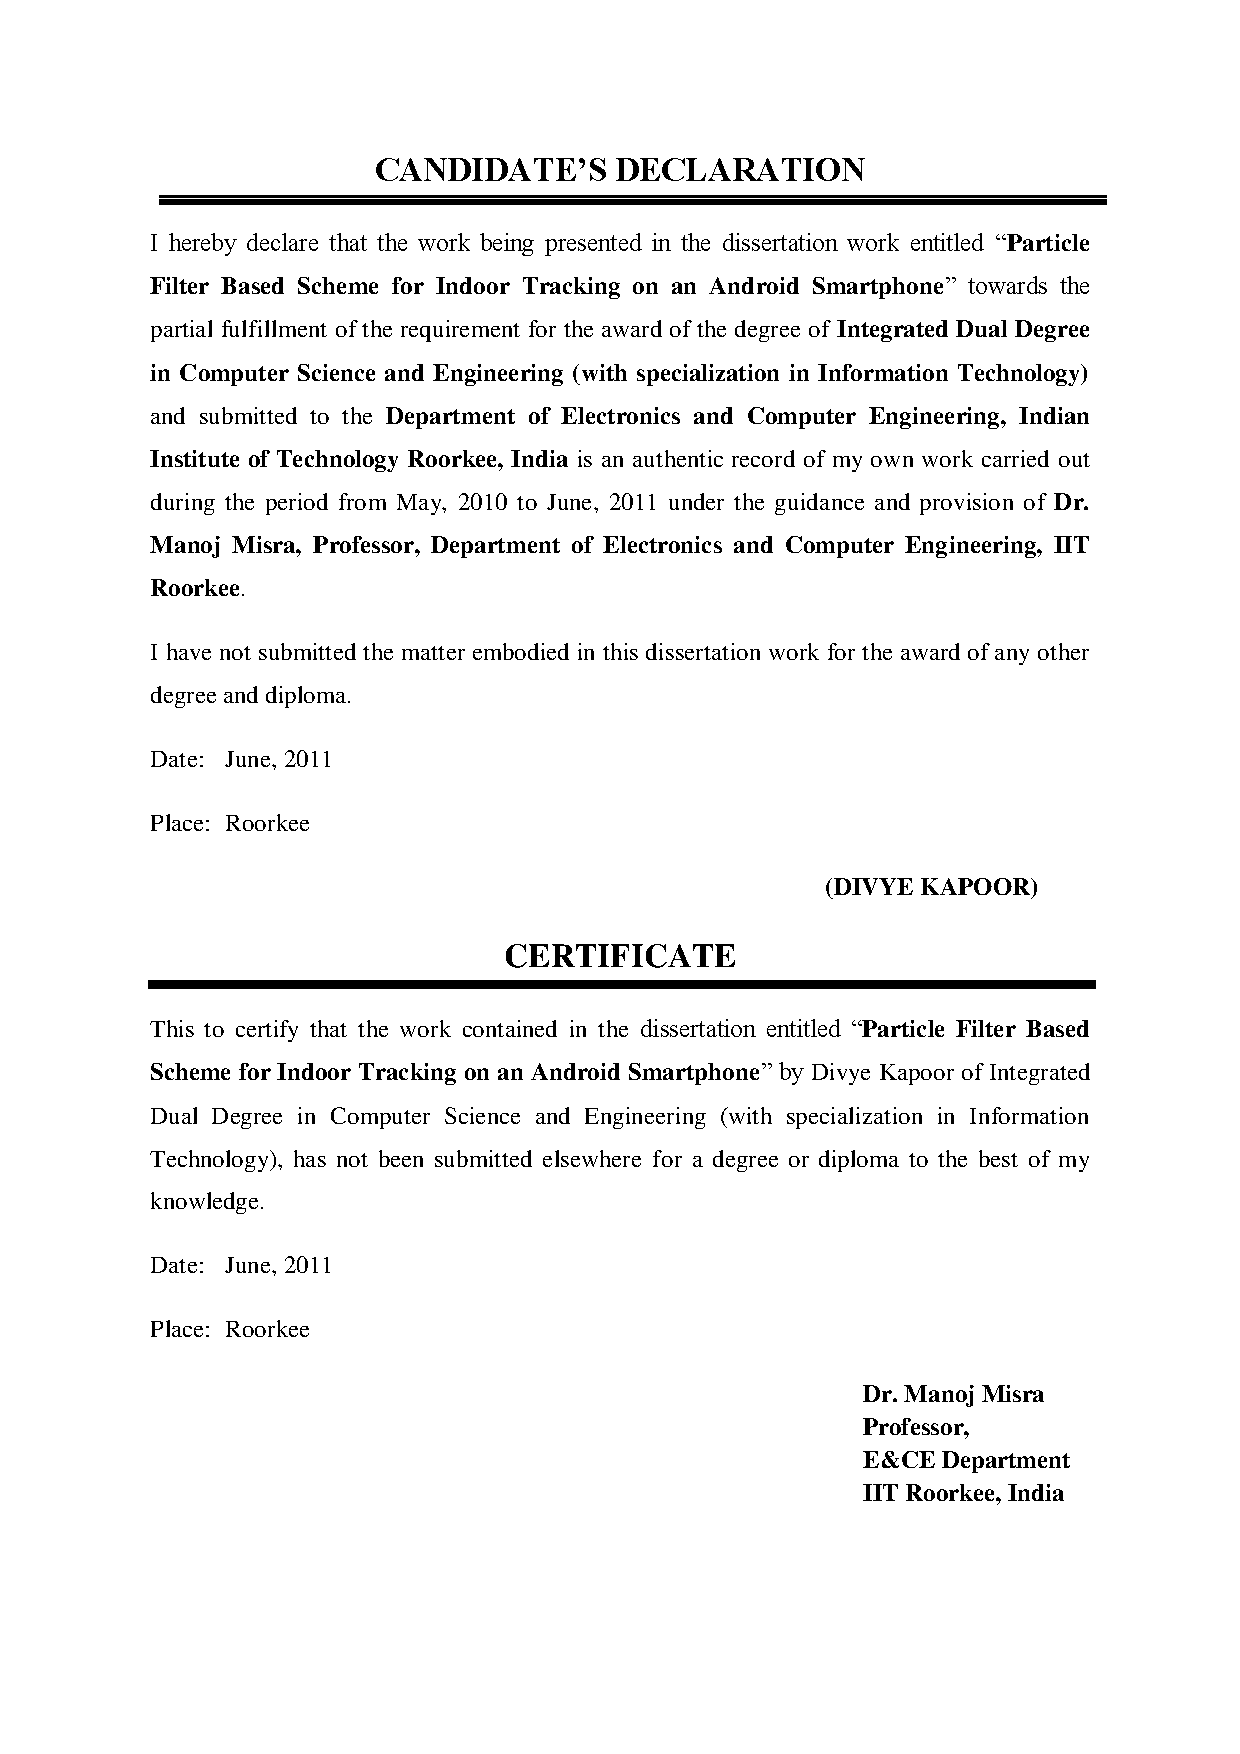
\includepdf{figures/candidate.pdf}

\chapter{Acknowledgements}

\onehalfspacing

I would like to take this opportunity to extend my most heartfelt gratitude to
my guide and mentor - \textbf{Prof. Manoj Misra}, Department of Electronics and
Computer Engineering, IIT Roorkee. His guidance, attention to detail and drive
for excellence have contributed greatly towards my education and also towards
ensuring that sterling work is done as part of my Masters dissertation. His
encouragement and unstinting faith have been essential in helping me learn, grow
and push the limits of my capabilities. I am fortunate to have been able to do
my dissertation under him.

My sincere thanks are due to \textbf{Dr. S. N. Sinha}, Professor and Head of the
Department of Electronics and Computer Engineering for providing the facilities
and hardware without which this thesis would have been all but impossible.
Thanks are also due to \textbf{Dr. Raheja}, Institute Architect, IIT Roorkee for
providing the blueprints of Ravindra Bhawan, the test site for this thesis. My
work would have been immensely more difficult without his help and cooperation.
The \textbf{Mahatma Gandhi Central Library} of IIT Roorkee also deserves a
mention in the Acknowledgements. They have provided unfettered access to the
world's highest quality research published in the IEEE and ACM journals. I have
always felt well supplied with information thanks to their hard work.

Sincere gratitude is also due to the authors of the many open source software
projects that have been very useful in the making of this thesis. The list of
projects is very long and it is impossible to name all, but I would like to give
a special mention to the authors and contributors of \textbf{\LaTeX, GNUPlot,
the GNU R Language, the GNU Core Utilities, Python, Linux, Android} and
\textbf{Eclipse}. This thesis is the result of standing on the shoulders of
giants and I am indebted to you for your efforts in maintaining such high
quality tools for the benefit of the world. Many many thanks.

Acknowledgements aren't complete without thanking \textbf{friends and family}.
They are the ones who have given unconditional encouragement and support. They
have shared my happiness on the days that things have worked and they have
helped get me through the days when things haven't. They have stood by me
through thick and thin and for that I am very grateful.



\chapter{Abstract}

The development of stable outdoor positioning and tracking algorithms has 
ushered in a new era of technology. Today GPS based navigators are 
ubiquitous and GPS based positioning and navigation has been integrated 
into smartphones. This has made life easy for navigation over large 
distances in an outdoor scenario. A new horizon for research has developed which
aims at providing that same ease of use in navigation 
and tracking in an indoor context.

Over the last few years, advances in technology have allowed for the 
development and integration of MEMS sensors into smartphones. These sensors 
(an accelerometer, a gyroscope and a magnetometer) can be leveraged to 
develop an indoor tracking solution. However, the resource constrained nature 
of smartphones necessitates modifications to prior work achieving the same 
in a non-mobile context. Additionally, the fact that 
the tracking device lies in a user's palm and not on a protected, stable 
surface (as is the case in robotics) generates a new set of challenges.

This thesis proposes and implements an online particle filter based algorithm for 
indoor positioning on an Android smartphone. The proposed algorithm 
is not only able to work well on the resource constrained device, it actually
yields an accuracy better than prior work in this area. Such results have 
been made possible by a careful approach to the problem with decisions made 
on factual data determined before and during the implementation of the 
proposed work. The final system is able to achieve a mean error of $0.5 m$
with a very low standard deviation value of $0.24 m$ and provides a clean,
intuitive tracked path. Results for comparison are produced using
a simple dead reckoning approach and a Nearest Neighbour 
Wifi corrected tracking algorithm. Both the algorithms are tested in the same
environment as the proposed work.



\tableofcontents
\clearpage

\listoffigures
\addcontentsline{toc}{chapter}{List of Figures}

\listoftables
\addcontentsline{toc}{chapter}{List of Tables}

\listofalgorithms
\addcontentsline{toc}{chapter}{List of Algorithms}

\clearpage
\listoftodos


\mainmatter

\onehalfspacing

\chapter{Introduction}

The world is an exciting place today. We are surrounded by technology that has
woven itself seamlessly into our lives. Today, many of us see the time on our
mobile phones, connect with friends and family through mobile versions of
popular social networks accessed through our smartphones. We talk to people
across the globe using that same mobile device and the smartphone doubles up as
a gaming console and eBook reader. The availability of a GPS sensor on 
smartphones has been a growing trend for the past few years and is now nearly
a de facto standard. Implementation of algorithms produced by researchers
over the past two decades on smartphones has resulted in tracking capability
that is quite accurate and suitable for navigation at outdoor locations. 
In fact, latest generation devices like the Samsung Nexus S even ship 
with a beta mobile application that doubles up as a standard car based GPS 
navigation device. So, while engineers at companies are working furiously 
to solve technical challenges for accurate tracking and navigation outdoors,
a different problem looms on the horizon: 

\begin{quote}
How do we take such tracking and navigational aids for mobiles indoors where GPS
based systems are virtually useless?
\end{quote}

This thesis will analyze this question and show multiple systems that 
provide indoor positioning and tracking using not much more than a
cutting edge smartphone. But before moving further, let me state my reasons
for picking this up as my dissertation proposal.


\section{Motivation}

For my dissertation, I wished to take up a topic that was current,
technologically intensive and had a broad scope of application. I had prior
exposure to location based services and map matching algorithms via my seminar
report\cite{SEMINAR} in 2010 and I was firmly convinced that Location Based
Services are going to play a very valuable part in the evolving future of mobile
devices. To enable a future that has relevant location based content, 
reliability of location of the user - both indoors and outdoors is a high 
priority. The outdoor location and tracking problem was being solved 
by using GPS, map matching and other filtering techniques. Long distance 
navigational aids were commercially available and the field is rather mature.
In contrast, the field of indoor positioning was highly fragmented, 
technologically diverse with no clear winners and few commercial offerings. 
The area was thus ripe for research.

\section{Potential Applications}

There are numerous potential applications for research in this area. Some are
obvious - Indoor navigation and tracking, applications as navigational aids for
the differently abled, and even location based services that aim to improve
customer experiences in malls and shopping complexes. However, some of 
the more interesting applications of this technology are in fields that 
are just opening up to research and implementation. 

\subsection{Navigational aids for the abled and differently abled}

Having a stable, highly accurate tracking solution is a prerequisite to 
provide navigational aids in unfamiliar surroundings like a customer at 
a mall or inside a huge departmental store. Visitors to huge office complexes
could also benefit with such navigational aids. The biggest beneficiaries
of such technology are the differently abled - who will be able to 
leverage such tools in coordination with highly mature devices customized 
to their needs so that they can move in indoor surroundings with just as 
much confidence as they do while using other navigational aids like GPS 
outdoors.


\subsection{Inventory tracking and retreival}

There are a number of large industries (eg. shipping industry, online ecommerce
vendors, private couriers, wholesalers etc.) that invest heavily in large
warehouses. One of their primary concerns is inventory management and retreival.
Most of the companies in these industries use some form of inventory tracking 
software that tracks what is present in the warehouses. They also evolve
conventions for storage that allow for easy retrieval of inventory. An indoor
tracking and navigation solution integrated with the inventory system can help 
workers easily and efficiently locate objects present in their warehouses and 
reduce incidents of misplacements or loss.

\subsection{Augmented Reality and Reality Fusion Gaming}

Among all the applications of indoor tracking - this is one that holds the 
greatest excitement.Augmented reality can be defined concisely as:
\begin{quote}
A technology that superimposes a computer-generated image on a user's view of
the real world, thus providing a composite view. (Adapted from \cite{SciDict})
\end{quote}

The field of AR is not new, however, technology has advanced to the point that
AR applications can now be built to run on smartphones while providing
exceptional engagement and interactivity. Researchers at Georgia Tech University
demonstrated such integration through a two player interactive AR game running
on an Android device at the 2010 Uplinq conference. The game was playable
anywhere provided a simple mat denoting the gaming area was placed on the floor.
The virtual characters (or sprites) were then created and layered on a camera
view of the mat. The two players could interact with the characters virtually
and their view of the sprites was altered in near real-time as they moved around
the mat. Another major application of AR to mobile devices has been shown by 
Layar wherein they overlay 3D models and informative content directly onto 
a user's view of a location. 

Integration of a stable indoor tracking solution with such AR applications will
allow the development of a new class of applications where a user's action and
location in real-life will correspond to a sprite's action in the virtual world
thus opening up arenas for AR based first person shooters etc. The possibilities
opened up by such technology are immense and limited only by imagination.

%\missingfigure{Show a typical AR image (sourced and cited)}

\section{Problem Statement\label{sec:problem_description}}
\todo{Please review}
All the applications mentioned above put different constraints of accuracy,
deployability, mobility and scalability on the tracking algorithm. We
concentrate on a specific type of the indoor tracking problem and thus limit
the scope of the thesis to the well defined problem statement below:

\begin{quote}
Develop and characterize a smartphone based particle filter sensor fusion
approach for online indoor tracking of pedestrians. 
\end{quote}


\section{Organization of the Thesis}

The thesis is split into various chapters for the convenience of the reader.

\begin{itemize}
\item Chapter \ref{chap:literature_review} details the flow of ideas and prior
work by researchers in this area.

\item Chapter \ref{chap:proposed_method} specifies the specific methods proposed
by the author for implementation of an indoor tracking system. The methods
detail the modifications proposed for implementation on a mobile device as well
as the choices guiding the approach.

\item Chapter \ref{chap:groundwork} specifies the field work that was done to
characterize the MEMS sensors and Wifi receiver on the smartphone and includes
the results of a project that implemented an indoor positioning system based on
the received signal strengths from different Wifi Access Points. This work was
done to determine a choice of suitable parameters for the algorithms specified
in Chapter \ref{chap:proposed_method}.

\item Chapter \ref{chap:implementation_details} discusses the implementation
details of the algorithms on an Android device and explains the architectural
organization of the entire codebase.

\item Chapter \ref{chap:results} discusses the performance of various components
of the solution and shows the performance of the final proposed method
contrasted with a naive dead reckoning approach and a Wifi based indoor tracking
approach.

\item Chapter \ref{chap:summary} finally summarizes the experiences derived from
the thesis and describes scope for future work in this area.

\item Additional test results which were
too voluminous to include in the main text of this thesis are present in 
the Appendix.

\item The papers and other sources of information used in this thesis are listed
in the bibliography at the end of this thesis.
\end{itemize}


\chapter{Literature Review}
 Done partially  in other files
\section{Research gaps}



%\chapter{Problem Description}
To develop and evaluate a high accuracy tracking system on a modern smartphone using sensor fusion techniques.



\chapter[Proposed Work]{Particle filter Based Map and Sensor Fusion technique for Indoor Tracking 
using an Android Smartphone\label{chap:proposed_method}}

\section{Relevant Prior Work}
As described in Chapter \ref{chap:literature_review} (Literature Review),
the pedestrian navigation system described in \cite{Wang} 
shows the most promise for accurate tracking of subjects in indoor tracking scenarios. 
The results of \cite{Evennou} which implements a similar system integrating an INS 
with Wifi data are very encouraging. However, we are cautioned 
against the computational complexity of a particle filter based solution and its attendant
implications while implementing the same on a mobile device by Evennou and Marx\cite{Evennou}. As we shall later
see, these cautionary words are well founded.

Our proposed method thus builds upon the work of Evennou and Marx\cite{Evennou}
and that of Wang et al\cite{Wang}. However many modifications specific to
implementation on a resource constrained device like an Android smartphone are
made. The proposed device for implementation is the Samsung I9020 (also called
the Samsung Nexus S which is co-branded with Google).

%Specifically, we discard the use of Wifi information for the central tracking
%algorithm and instead use it only in the error recovery phase. The justifications
%for these modifications are made in the accompanying text.
%modifications are proposed and implemented to take into account the fact 
%that our implementation system is an Android smartphone with a number of 
%sensors and limited processing capabilities. 

%The device that is the test-bed for implementation is the Samsung Nexus S. 
%The onboard accelerometer, magnetometer and gyroscope of the Nexus S are used 
%as inertial navigation sensors. The algorithm is then analyzed with different 
%parameters and paths and is compared and contrasted with two other tracking 
%approaches implemented on the same device - one a simple uncorrected dead
%reckoning implementation and the other a pure Wifi based based tracking system.
%These results are summarized in Chapter \ref{chap:results}.

\section{System Inputs\label{sec:system_inputs}}

Given the choice of hardware, we are constrained to use only specific 
data sources for our algorithm. 
The sensors available on a typical Android Smartphone are:
\begin{enumerate}
\item A 3-axis accelerometer for measuring acceleration of the device.
\item A 3-axis magnetometer for measuring the surrounding magnetic field.
\item A gyroscope for providing angular velocity information.
\item A camera for providing visual information.
\item A Wifi Network Card with the ability to provide measurements of the received signal strengths. (RSSI)
\end{enumerate}

Besides the sensors mentioned above, additional sources of information 
that we can make available to the system are:

\begin{enumerate}
\item Map information detailing the test environment.
\item A site survey of the test environment which provides Wifi location fingerprints augmented by 
    orientation information of the reciever when the fingerprint was taken.
\end{enumerate}

Characterizations of these data sources as well
as other relevant parameters will be done as ground-work in 
Chapter \ref{chap:groundwork}.

\section{Device Limitations\label{sec:device_limitations}}

Being a resource constrained device, a number of limitations are imposed on 
software for these systems. Some of the ones most affecting the implementation
are:

\begin{itemize}
\item Applications are restricted to a maximum memory utilization of 16 MB on 
    older devices and newer devices get limits based on the size of their 
    RAM. The Nexus S has a maximum limit of 32 MB, other devices usually have
    lower limits of 24 MB or 16 MB.
\item The CPU usage of the application has to be controlled. Applications 
    that use the CPU intensively for more than a few seconds are detected as 
    misbehaving applications and the user is prompted to kill them.
\item Sensor events are dropped if the event delivery thread is busy processing
    the last delivered event. This puts significant limits on the 
    amount of inter sample processing that may be performed while 
\end{itemize}


\section{Background on Particle Filters}
\todo{What/How much to write here and where to put in the thesis?}
Particle filters belong to a class of Sequential Monte Carlo algorithms 
that depend essentially approximating a probability distribution function based
on a Monte Carlo simulation of the system using observation samples. Particle 
filters have been known to be very useful for tracking in systems where joint
probability distribution functions are either not completely known or hard 
to sample. 

In this case, our problem of indoor tracking is essentially the 
determination of a latent variable $x_t$ which represents the position of the 
user after we receive a series of observations ($o_0 \dots o_t$) from the 
sensors on the Android device. Effectively, we wish to approximate the the 
probablity distribution $p(x_t|o_t,o_{t-1}\dots,o_0)$ at any time instant $t$
so that we may determine the position of the device using the expectation 
function $E[x]$ on the probability distribution $p(x_t|o_t,o_{t-1}\dots,o_0)$
and we wish to use a particle filter to help us do so.

Particle filters are a huge topic in and of themselves. Thus, in the interests
of brevity, the reader is referred to the excellent expositions of particle 
filters for tracking applications in \cite{Ristic} and to \cite{Arulampalam}
for particle filters in the context of non-linear, non-gaussian Bayesian
tracking.


\section{Proposed Method}

Keeping the availability of the inputs described above as well as the device 
limitations described in Section \ref{sec:device_limitations} in mind, a less 
computationally intensive method is proposed in 
Algorithm \ref{algo:proposed_method}.

\begin{algorithm}
\dontprintsemicolon
\SetKwInOut{Input}{Input}
\Input{Sensor Events from device sensors}
\KwResult{An estimate of the location of the device at any time through the variable $L$}
\Begin{
    $L \longleftarrow FirstFix()$ \;
    $P \longleftarrow$ $N$ particles around $L$ corrupted by gaussian noise\;
    \ForEach{$stepEvent$ from $sensors$}{
        $P' \longleftarrow ApplyDynamicalEquations(P)$\;
        $P' \longleftarrow MapSelect(P', P)$\;
        \eIf{$P'$ is $\emptyset$}{
            $R \longleftarrow PerfomRecovery(P)$\;
            \If{$R$ is not $\emptyset$}{
                $P \longleftarrow R$
            }
        }{
            $P \longleftarrow P'$\;
        }
        Resample set $P$ uniformly to a fixed sized set and
        corrupt the new particles thus generated with gaussian noise\;
        $L \longleftarrow Mean(P)$\;
    }
}
\caption{High Level View of the System\label{algo:proposed_method}}
\end{algorithm}

Algorithm \ref{algo:proposed_method} is very general. Also, though it is 
stated in a sequential manner, the it needs to 
be implemented in an event-driven fashion to allow for online tracking. 
The \textbf{ForEach} loop in the algorithm is essentially an event loop 
that depends on step detection.

Procedures to determine \emph{FirstFix}, detect steps from sensor data, 
\emph{MapSelect}, \emph{ApplyDynamicalEquations}, and \emph{PerfomRecovery} are explained
below.

%\begin{enumerate}
%\item A first-fix position estimate will be taken by means of manual input or 
%    via QRCodes through the smartphone camera.
%\item A step counting approach in accordance with a modified peak and 
%    valley approach and a step stride estimation in accordance with
%    \cite{ADXL202} will be used.
%\item A low complexity particle filter is used to implement the tracking 
%    algorithm. 
%\item Map information is used to provide means for correcting drift in the 
%    simple tracking algorithm.
%\item Additional "hidden" variables are used in the dynamical equations of the 
%    system to compensate for a constant sensor drift and small variations in 
%    the step size of the user. 
%\end{enumerate}

Comparison of the proposed method will be done with 2 other algorithms, also
implemented on the smartphone: 

\begin{enumerate}
\item A simple step based dead reckoning solution that directly uses sensor data.
\item A simple step based dead reckoning solution with a Wifi based nearest neighbour algorithm incorporated as a 
    drift correction method.    
\end{enumerate}

These algorithms are being implemented as control algorithms for comparisons
in order to provide suitable comparative information since maps and test 
environments differ substantially and make comparative analysis difficult.

\section{First Fix\label{sec:first_fix}}

Dead reckoning refers to a method of position determination where the current
location is estimated based on a known starting location and offsets from the
known location measured via instruments.

For any dead reckoning algorithm, it is important to provide a good starting
point. Low error in the starting location contributes to better performance.
Our proposed method is based on the dead reckoning concept and thus requires 
a (reasonably) accurate starting point (also called a first fix).

In order to provide the starting point to the algorithm two approaches are 
proposed:

\begin{enumerate}
\item Directly choose the starting location on a map using the capacitive 
    touchscreen
\item Select the starting location based on QRCode recognition using the onboard
    camera. The QRCodes were printed and pasted at specific locations 
    in the test environment and the user is required to simply take a 
    picture of it using the onboard camera.
\end{enumerate}

\subsection{QR Codes\label{sec:QRCodes}}
QRCodes are a kind of 2 dimensional machine readable code (an example of which
is shown in Figure \ref{fig:sample_qrcode}). The information encoded in this
format can be read off by processing an image acquired from a camera. 

QRCodes can contain a variety of content - 
from URLs to Contact information. They can also contain plain text. 

For this application, we use the plain text information mode of QRCodes 
to provide encoding of a human-readable text representation of map points. 
This human and machine readable representation is achieved with the lightweight
JavaScript Object Notation (JSON) representation. 
Details of the format chosen for this application are
mentioned below:

\begin{figure}
    \centering
    \includegraphics[width=3in]{figures/sample_qrcode}
    \caption{A Sample QRCode\label{fig:sample_qrcode}}
\end{figure}


\subsubsection{QR Code information format}

A typical format used for storing all the relevant information in a QRCode is
shown in Figure \ref{fig:QRCode_info_format}. As is proper for any data 
serialization format, it stores a Version number and a Type field to 
distinguish itself from other data serialization formats. It also includes
critical information about the point itself - the X and Y locations on 
the relevant map as scaled on a 0-1 scale. A full description of the fields
is given in Table \ref{tbl:QRCode_fields_table}.

The fields are descriptive 
and quite human readable. However, because they are in JSON, a basic 
check of well-formedness can be made by programs. The data format retains 
extensibility as it is able to accommodate additional fields which will
be ignored by applications that are not built to expect the presence of those
fields.

\begin{figure}
    \centering
\begin{verbatim}
{
   "Version": 1,
   "Type": "MapPoint",
   "MapURL": "http://www.iitr.ernet.in/path/to/sample/map.png",
   "Scale": 0.010716161,
   "X":0.70625,
   "Y":0.16479166666666667 
   
}
\end{verbatim}
    \caption{A sample data point encoded as text information in a QRCode\label{fig:QRCode_info_format}}
\end{figure}

\begin{table}
\centering
\begin{tabular}{p{1in} p{4in}}
\hline
\hline
Field Name      &       Field Description \\
\hline
Version         & Constant value 1. May be incremented if additional fields are added to the format. \\
Type            & Represents the type of QRCode waypoint sample that was just acquired. Type "MapPoint" indicates that the QRCode represents a point on a Map. Alternative and  additional information can be provided by choosing other Types. For example,  a Type of "WifiAP" could be used to provide location information about  Wifi Access Points in the surroundings. \\
MapURL          & This field always refers to a publicly available map associated with the environment where  the QRCode was pasted. A png map type has been indicated, but any other resource type that  a client is able to handle should be accepted. \\
Scale           & Scale is an optional parameter of a MapPoint. It represents the scaling factor between distances on a map with distances in the real world. It can be omitted if it is expected that the  client will have some other way of figuring out the scale of the map based on information encoded within the map itself. \\
X and Y         & These are values encoded in the real range [0-1] which represent the location of the QRCode on a map referred by it. These values are used for providing a first fix to the  reckoning algorithms.  \\
\hline
\end{tabular}
\caption{Explanation of the fields used in the QRCode Information Format\label{tbl:QRCode_fields_table}}
\end{table}

\section{Noise filtering\label{sec:NoiseClamping}}

It is well known that while measuring real world information, most sensors
 pick up noise from the environment that affects the readings of the 
sensed variables. The MEMS accelerometer present on a typical smartphone is 
no different. 

In general, we assume that the accelerometer sensor noise is below a small 
threshold $T$ when the device is static on a firm surface such as a table. 
A higher threshold $Q$ is required when the device is being kept at the palm of 
a hand because of small noisy variations introduced by the palm itself.

The filtering process uses a simple clamping mechanism. The filter 
rejects a reading of the accelerometer based on the following constraints:

\begin{equation}
NoiseFilter(a_i) =  \begin{cases} 0 & \text{if $|a_i| \le Q$,} \\
                                a_i & \text{otherwise}
                    \end{cases}
\end{equation}

The values of T and Q are determined as part of the groundwork in Chapter 
\ref{chap:groundwork}.

The filtering process is very important for the step counting algorithms
to detect accurate peaks.

\section{Distance Estimation}

The acceleration of the human body as part of the act of walking is small and 
very impulsive in nature. Unfortunately, the linear acceleration values
produced by it are so small that they are virtually indetectible from the 
sensor noise of the MEMS accelerometer of the Android device. However, the 
act of putting a foot on the ground generates an impulse along the Z 
axis of the accelerometer which is clearly distinguishable in the sensor 
readings. Thus, we use the step count method described in
\cite{Wang} and \cite{Ladetto} to detect motion of the user holding the device.

By relating the acceleration impulses to the size of a step, 
an inertial navigation system may be created. An empirical formula 
from \cite{ADXL202} is used to estimate step sizes from the readings sensed by
the accelerometer. Details of all the methods used to achieve the same 
follow:

\subsection{Step detection procedure\label{sec:step_detection}}

\subsubsection{Zero Crossings}

This step counting method is described in \cite{Wang} is based on a similar 
method devised for outdoor pedestrian navigation by \cite{Ladetto}. It is a
simple formulation that counts the number of zero crossings of a 
filtered version of the raw accelerometer signal which represent double the 
number of steps taken. However, this method, when implemented, generates 
step events at zero crossings which correspond to a body in motion.
Since each step has to be associated with an angle of motion, it might be 
advantageous to ensure that step events are associated with points where 
the foot of the user is on the ground, leading to better stability of angle 
readings. Thus, the Peak and Valley hunting method is also proposed. 

\subsubsection{Peak and Valley hunting\label{sec:peak_and_valley}}

The Peak and Valley hunting procedure is an alternate method being
proposed for step detection.
This method will detect the same number of crossings as the zero crossing 
method but will raise the step events whenever the foot of the user 
strikes the ground for the beginning of the next step. 

In this method a 2-state machine is constructed according to Table
\ref{tbl:peak_valley_state_table}. This method outputs a detected step at 
the first positive peak in the accelerometer sensor data that corresponds to 
the beginning of the next step. Also, since it only processes data at 
points where the first derivative of the accelerometer signal is zero and 
the accelerometer signal itself is non-zero, it can reduce computational 
effort for cases where zero crossing would perform considerable testing
on account of being at the value 0, waiting for a transition. Additionally,
the values of $A_{max}$ and $A_{min}$ that will be required later are 
updated only during these intervals, thus saving further computational 
resources compared the Zero Crossing method. The disadvantage of this method
though is the additional lag introduced between a step being taken and its 
event being delivered to the application.

\todo{Improve this area}
\begin{table}[h]\centering
    \begin{tabular}{c p{1in} c p{2.7in}} \hline
    State & Accel. Value     & New State &  Action\\     \hline
    $q_0$ & Positive Peak ($P$) Detected  & $q_1$     & Update $A_{max}$ if peak $P > A_{max}$. Output a step event if $flag = 1$. Reset $flag$ to 0.  \\ 
          & Other values            & $q_0$     & Ignore \\         \hline
    $q_1$ & Negative Trough ($T$) Detected & $q_0$    & Update $A_{min}$ if $T < A_{min}$. Set $flag$ to 1. \\
          & Other values            & $q_1$     & Ignore \\ \hline
    \end{tabular}
    \caption{State table of the step detection state machine\label{tbl:peak_valley_state_table}}
\end{table}

\subsection{Step Size Estimation}

Engineers from Analog Device have published an empirical relationship between 
acceleration values and step size in \cite{ADXL202}:

\begin{equation}\label{eq:step_size}
 Step-size = C \sqrt[4]{A_{max} - A_{min}}
\end{equation}

The constant $C$ is a scaling factor that is used as a constant of proportionality
to scale the step-values to real world distances and $A_{max}$ and $A_{min}$
represent maximum and minimum acceleration values corresponding to the 
peaks and troughs associated with a step. 

This equation is used to obtain an estimate of the step size when a user 
takes a step.

\subsection{Determining the Training Constant}

The training constant for each user was determined experimentally. 
Users were asked to perform a short walk between 2 QRCoded locations
present in a straight line along a corridoor.
Since, the QRCodes represent fixed locations in the real world, the actual 
distance between them can be found using simple Euclidean geometry. From 
simple step counting, we are able to figure out the number of steps taken.
Also, by means of the step size formula mentioned in \eqref{eq:step_size},
we can estimate the distance travelled based purely on the accelerometer
values. We can then find the training constant by simply plugging in 
the values into the following equation:

\begin{equation}
C=\frac{\sqrt{(x_{2}-x_{1})^{2}+(y_{2}-y_{1})^{2}}}{\sum_{i=1}^{stepcount}\sqrt[4]{(A_{max_{i}}-A_{min_{i}})}}
\end{equation}

Here,\\
\begin{tabular}{l l}
$C$                         & is the training constant   \\
$(x_1, y_1), (x_2, y_2)$    & are the anchor point locations provided by the QRCodes \\
$A_{max_{i}}, A_{min_{i}}$  & represent the maximum and minimum \\
                            & acceleration values corresponding to the $i^{th}$ step.\\
$stepcount$                 & The number of steps detected by the algorithm in section \ref{sec:step_detection} \\
\end{tabular}


\section{Dynamical Equations for the System}

With the preliminaries now out of the way, we can develop the dynamical model
of our proposed solution. The basic step update equation for the system 
can be written as:

\begin{equation}\label{eq:dr_eq}
\begin{bmatrix}x_{i+1}\\
y_{i+1}
\end{bmatrix} = \begin{bmatrix}x_{i}\\
y_{i}
\end{bmatrix}  + d{}_{i} \begin{bmatrix}-cos(\theta_{i})\\
sin(\theta_{i})
\end{bmatrix} 
\end{equation}

Here,\\
\begin{tabular}{p{1in} p{4in}}
$x_i, y_i$          &   represent location of the device after the $i^{th}$ step\\
$x_0, y_0$          &   are the first fix values obtained via the methods of Section \ref{sec:first_fix}\\
$d_i$               &   the predicted step distance as per the step estimate equation \eqref{eq:step_size}\\
$\theta_i$          &   the angle associated with the detected step based on a magnetometer reading\\
\end{tabular}

These equations are written assuming a coordinate system for the map where the 
origin is at the top left corner of the map, the $x$ axis being
positive towards right and $y$ axis positive downwards with $TrueNorth$ of the map
pointing upwards. Effectively, equation \eqref{eq:dr_eq} represents a raw dead reckoning
solution. Unfortunately, these equations do nothing to counteract the biggest
disadvantage of dead reckoning: unbounded error growth. The dynamical
representation is also overtly simplistic because it fails to take into account
other issues such as sensor drift and sensor bias. The magnetometer is the
biggest culprit in this regard as it is highly sensitive to stray magnetic
effects in the environment.

\subsection{Modelling Orientation Sensor Noise}

\begin{equation}
\begin{bmatrix}x_{i+1}\\
y_{i+1}
\end{bmatrix} = \begin{bmatrix}x_{i}\\
y_{i}
\end{bmatrix}  + d{}_{i} \begin{bmatrix}-cos(\theta_{i}+\vartheta)\\
sin(\theta_{i}+\vartheta)
\end{bmatrix} 
\end{equation}

We modify the dynamical equation to add an additional parameter $\vartheta$
which is a random variable that represents random variations akin to white noise
in the reading from the true value of the magnetometer. $\theta_i$ now
represents the true angle associated with the step motion.

\subsection{Accounting for Orientation Sensor Bias\label{sec:angle_bias}}

Angular readings from the magnetometer often turn out to be biased from
$TrueNorth$. This bias can creep in due to 2 different reasons - the first being
specific, environmental magnetic fields which distort the actual detection of
$TrueNorth$ in the system and the second being a bias that creeps in due to the
way the user holds the smartphone in the palm of his hand and the offset thus
produced. To take into account such offsets, we modify the dynamical equations
as follows:

\begin{equation}
\begin{bmatrix}x_{i+1}\\
y_{i+1}\\
\theta_{b_{i+1}}
\end{bmatrix} = \begin{bmatrix}x_{i}\\
y_{i}\\
\theta_{b_i}
\end{bmatrix}  + \begin{bmatrix} d{}_{i} & d_i & 1 \end{bmatrix} \begin{bmatrix}-cos(\theta_{i}+\theta_{b_i}+\vartheta)\\
sin(\theta_{i}+\theta_{b_i}+\vartheta)\\
\theta_t\\
\end{bmatrix} 
\end{equation}

\begin{equation}
\theta_t \sim \mathcal{N}(0,\sigma_{angle})
\end{equation}

In this modified version of the dynamical equations, we have added a slowly
varying term $\theta_{b_i}$ that represents an explicit bias in the readings
from the magnetometer at the time of the $i^{th}$. This bias value is updated at
each step by altering it with a small gaussian noise of zero mean an a variance
determined by the characteristics of the magnetometer. The choice of
$\sigma_{angle}$ was made on the basis of the groundwork done. Corrections
for the sensor bias will be made when $MapSelect$ is applied to the particles by
the overall algorithm.

\subsection{Accounting for Varying Step Sizes and Missing Steps\label{sec:step_bias}}

The second issue at hand is step size variation and missing steps. Steps may
be missed by the step detection procedures or phantom steps may be detected
due to sensor noise or other events. Changes in step sizes due to changes in 
footwear or floor material as well as the leads and lags produced due to a 
slightly incorrect calibration constant also contribute to deviations of 
apparent distance travelled versus the apparent distance travelled. To account
for this bias in step size detection, we introduce an additional parameter
$d_{b}$ in the dynamical system that accounts for the step bias. 
Thus, the new equations for the dynamical system are:

\begin{equation}
\begin{bmatrix}x_{i+1}\\
y_{i+1}\\
\theta_{b_{i+1}}\\
d_{b_{i+1}}\\
\end{bmatrix} = \begin{bmatrix}x_{i}\\
y_{i}\\
\theta_{b_i}\\
d_{b_i}
\end{bmatrix}  + \begin{bmatrix}(d{}_{i}+d_{b_i}) & (d{}_{i}+d_{b_i}) & 1 & 1\end{bmatrix} \begin{bmatrix}-cos(\theta_{i}+\theta_{b_i}+\vartheta)\\
sin(\theta_{i}+\theta_{b_i}+\vartheta)\\
\theta_t\\
d_{t}
\end{bmatrix} 
\end{equation}

\begin{equation}
d_{t} \sim \mathcal{N}(0, \sigma_{step})
\end{equation}

In this representation, $d_{b_i}$ is a slowly varying bias variable on the step
size and the gaussian variance used during each update step is $d_t$. The 
determination of the variance of $d_t$ again depends on sensor to sensor and 
is evaluated empirically for our system to be close to $step\_size/25$.

Note that the equations mentioned in Sections \ref{sec:angle_bias} and
\ref{sec:step_bias} will work only if the map information is dense enough to
eventually eliminate groups of particles with incorrect orientations and 
step drifts. Otherwise, the only effect of maintaining the bias variables will 
be to slightly increase the variance of the variables $x_i$ and $y_i$.
An explanation of how these bias variables actually help determine overall
angle and step bias is provided in Section \ref{sec:overall_bias}

\subsection{Ensuring particle diversity}

The presence of the variables $\theta_{t}$ and $d_t$ represents an 
intentional introduction of randomness into the system to ensure 
particle diversity. For example, if two particles start out with the same
state vectors, say 
$ [ x_i y_i \theta_{b_i} d_{b_i} ] $ and 
$ [ x_j y_j \theta_{b_j} d_{b_j} ] $, they will in the immediate 
next time step tend to diverge due to possibly different samples of the 
random variables $\theta_{t}$ and $d_t$. So, 
when evolved over a large number of steps, similar samples will take 
slightly different paths through the state space, thus ensuring particle 
diversity of the particle filter. Note however, that the choice of 
magnitudes of the variance of $\theta_t$ and $d_t$ is critical. If the 
values chosen are too small, states that were possible physically are 
not achieved by the particle filter and if the values chosen are too large,
computational effort will be wasted for unachievable states. For our case 
of a highly resource constrained machine, this is very undesirable for we
wish to maximize the effectiveness of our particles. In this regard, it is 
also very advantageous if we have a highly detailed map of the area for 
unachievable states are quickly pruned and computational effort is 
redirected towards states with more likelihood. The integration of 
map information is described in the subsequent section.

\section{Integrating Map Information}

Map information can be integrated into the system in a number 
of ways. The simplest way to use map information as a selection 
function which is similar to \cite{Wang}:

\begin{equation}\label{eq:select}
MapSelect(p_{i+1}, p_i) = \begin{cases}1 - P_{wall} & \text{if $p_i + \alpha (p_{i+1} - p_i)$ for $\alpha \in [0,1]$} \\
                                                    & \text{does not cross a wall}\\
                                    P_{wall} & \text{otherwise}
                          \end{cases}
\end{equation}

Here,\\
\begin{tabular}{p{1.5in} p{3.5in}}
$p_{i+1}$ and $p_i$ &   are tuples corresponding to map locations ($x_{i+1}$, $y_{i+1}$) and ($x_i$, $y_i$) respectively. \\
$P_{wall}$ &   represents the probability of selection of the particle if it crosses a wall. \\
$\alpha$ & is a parametric variable used to represent a line between the two points $p_{i+1}$ and $p_i$ \\
\end{tabular}

Wang et all\cite{Wang} suggest that a $P_{wall}$ of 0 be used as such a motion
is impossible. Though simplistic, this approach works well by swiftly removing
unreachable particles. It is very light computationally too. However, given our
very limited budget for particles, it might not be prudent to remove a particle
simply because it was crossing a wall very close to a door. Thus, more advanced
map integration techniques may well be envisaged with $P_{wall}$ varying based
on the distance of the intersection point from the closest door in the wall. 

\section{Determination of overall orientation and step biases\label{sec:overall_bias}}

The integration of map information with the dynamical equations of the system 
via a selection function $MapSelect$ allows us to actually determine 
the extent of orientation and step bias. The idea behind it is simple. 
However, before explaining it, let us define the following two terms:
\begin{equation}
\displaystyle
\theta_b = \frac{1}{N}\sum\limits_{i} \theta_{b_i}
\end{equation}

\begin{equation}
\displaystyle
d_b = \frac{1}{N}\sum\limits_{i} d_{b_i}
\end{equation}

Here,\\
\begin{tabular}{p{1.5in} p{3.5in}}
N & is the total number of live particles in the system \\
$d_{b_i}$ and $\theta_{b_i}$ & retain their meanings from the previous sections \\
$\theta_b$ & represents overall system orientation bias at the $i^{th}$ stage \\
$d_b$ & represents overall system step bias at the $i^{th}$ stage \\
\end{tabular}

When no walls exist in the vicinity of the particles, map information is sparse
and few particles are eliminated because of it. Thus, we have insufficient 
feedback from our system to determine the value of orientation bias ($\theta_b$)
as all positions are equally valid. However, in a confined space like a 
doorway or a corridoor, there exist only a few valid range of angles over 
a sequence of steps. Thus
errant particles will be swiftly rejected by $MapSelect$ and we will 
get a highly accurate estimate of the degree of orientation bias present 
in our system.

The justification for step bias ($d_b$) lies similarly in the fact that while
moving along corridoors, we will have accumulated
a certain degree of step drift. This drift ensures that we are slightly 
uncertain of our exact position along the corridoor after walking through it for a long time
as we have not received any feedback from $MapSelect$ along our direction of motion. 
Thus,
some particles representing our location will be further along the corridoor than others and we have no way 
to choose between them other than by treating them at par. However, 
whenever we make a sharp turn on the map, the presence of walls and other 
obstacles immediately before and after the junctions on the map will cause 
a number of particles to be rejected by $MapSelect$. The values of $d_{b_i}$
remaining represent the net bias in the step size of the system. Thus,
their mean $d_b$ is a good representation of the step bias of the system.

\section{Recovering from particle insufficiency}

Particle insufficiency is a weakness of particle filters. It arises if 
no valid successor states $p_{i+1}$ can be found from the current set of 
particles $p_i$ when the observation $o_i$ is taken into account and applied 
to the dynamical equations of the system. (That is, all successor states 
$p_{i+1}$, have $MapSelect(p_{i+1}, p_i) = 0$). This possibility is 
further accentuated in resource constrained systems like ours which 
have a hard limit on the maximum number of particles that can be 
updated between two steps (since the algorithm is working in an online
fashion with a location estimate being available after every step).

The insufficiency of particles can be handled by a number of ways. 
The simplest one is: increase the number of particles being updated at each 
step and ensure enough particle diversity so that you always have 
a few particles that survive incorrect decisions of the particle filter. 

Widyawan \cite{Widyawan} suggests an alternative method: maintaining particle
history information so that an incorrect decision of the particle filter can be
rolled back a few steps in the past and an alternative decision can be made that
does not cause the particle filter to suffer particle insufficiency. However,
the method suggested is expensive in terms of memory usage and computational
cost.

The recovery algorithm ($PerformRecovery$) being proposed is stated in 
Algorithm \ref{algo:recovery}.

\begin{algorithm}
\dontprintsemicolon
\linesnumbered
\SetKw{Break}{break}
\SetKwInOut{Input}{Input}
\Input{A set of particles $P$ such that $ApplyDynamicalEquations(P)$ yields $\emptyset$, $\sigma_X$ and $\sigma_Y$ are the positioning errors of the Wifi based positioning system}
\KwResult{A new set of particles $R$ which approximate the location of the device or $\emptyset$}
\Begin{
    \emph{Try to recover by finding particles in the surroundings by random sampling}\;
    $retryCount \longleftarrow 0$\;
    \While{$retryCount < MaxRetries$}{
        \For{$j$ in $[1..N]$}{
            $r_j \longleftarrow (\mathcal{N}(0, \sigma_X), \mathcal{N}(0, \sigma_Y))$\;
            $selectParticle \longleftarrow false$\;
            \ForEach{$p_i \in P$}{
                \If{$MapSelect(r_j, p_i)$}{
                    $selectParticle \longleftarrow true$\;
                    \Break\;
                }
            }
            \If{$selectParticle$ is $true$}{
                $R \longleftarrow R \cup \{ r_j \}$\;
            }
        }
        $R' \longleftarrow ApplyDynamicalEquations(R)$\;
        \If{$R'$ is not $\emptyset$}{
            \Return $R$\;
        }
        $retryCount \longleftarrow retryCount + 1$\;
    }
    \emph{We have failed to find suitable particles by random sampling, fall back on Wifi}\;
    $wifiLocation \longleftarrow PerformWifiPositioning()$\;
    \For{$j$ in $[1..N]$}{
        \emph{Corrupt the wifi location with gaussian noise to approximate the error}\;
        $r_j \longleftarrow wifiLocation + (\mathcal{N}(0, \sigma_X), \mathcal{N}(0, \sigma_Y))$\;
        $R \longleftarrow R \cup \{ r_j \}$\;
    }
    $R' \longleftarrow ApplyDynamicalEquations(R)$\;
    \eIf{$R'$ is not $\emptyset$}{
        \Return $R$\;
    }{
        \emph{We've failed to find suitable particles, return failure and handle it by skipping the step information.}\;
        \Return{$\emptyset$}\;
    }
}
\caption{Recovery algorithm for particle insufficiency\label{algo:recovery}}
\end{algorithm}

There are a few interesting things to note about the recovery algorithm.
The first being that it retries finding suitable particles. This is an 
optimization as we don't want to spend too much effort at recovering 
unless we really have to since the inner algorithm has an O($N \times |P|$) 
complexity. In case we fail to recover directly from random sampling 
around the location, we retry with Wifi Positioning data. If that fails 
too, then we return an empty set. The system handles this failure by skipping 
the step event (discarding it as possibly invalid sensor readings).

\section{Summary}

The above algorithms represent a lower complexity particle filter that 
is proposed to be suitable for implementation on resource constrained 
smartphones. The performance of the proposed methods is analyzed in 
Chapter \ref{chap:results}.



\chapter{Groundwork\label{chap:groundwork}}

\todo{Figures for this entire chapter have to be rebuilt}

Before implementing any system, it is imperative to understand the data at hand
so as to make correct analytical decisions. In this regard, groundwork was done
to characterize all the input data sources.

\section{Hardware}
The hardware used to produce the results is the Samsung Nexus S (cobranded with
Google) running Android 2.3.4. The official specifications of the device can be
obtained from the manufacturer's website [link to website with reference] A
short listing of the sensors present on the device is given below based on how
the device reports the sensors via the software APIs:

\begin{enumerate}
\item KR3DM 3-axis Accelerometer
\item AK8973 3-axis Magnetic field sensor
\item AK8973 Orientation sensor
\item GP2A Light sensor
\item GP2A Proximity sensor
\item K3G Gyroscope sensor
\item Gravity Sensor
\item Linear Acceleration Sensor
\item Rotation Vector Sensor
\item An 802.11 b/g/n compatible Wifi NIC
\end{enumerate}

It may be noted that of these sensors, the Gravity sensor, the Linear
Acceleration Sensor and the Rotation Vector Sensor are derived sensors. They
depend on filtering the raw data sensed via the accelerometer and the
magnetometer to generate their sensed values. In essence, the Gravity sensor is
a low pass filter over the accelerometer values (since gravity is essentially
stable for the device at a particular orientation), the Linear Acceleration
Sensor is a high pass filter over the accelerometer values (the high frequency
changes in acceleration are presumed to occur due to device motion and thus
correspond to linear acceleration of the device) and the Rotation Vector Sensor
is a composite sensor that fuses Gravity information derived from the
3 axis Accelerometer and the magnetic field information derived from the
3 axis Magnetic field sensor to orient the device in the 3 Dimensional World 
Coordinate space. The actual method used to do so is described in the API
documentation \cite{AndroidSensorManager} and
further discussion is out of scope for this thesis.

\begin{figure}
\centering
    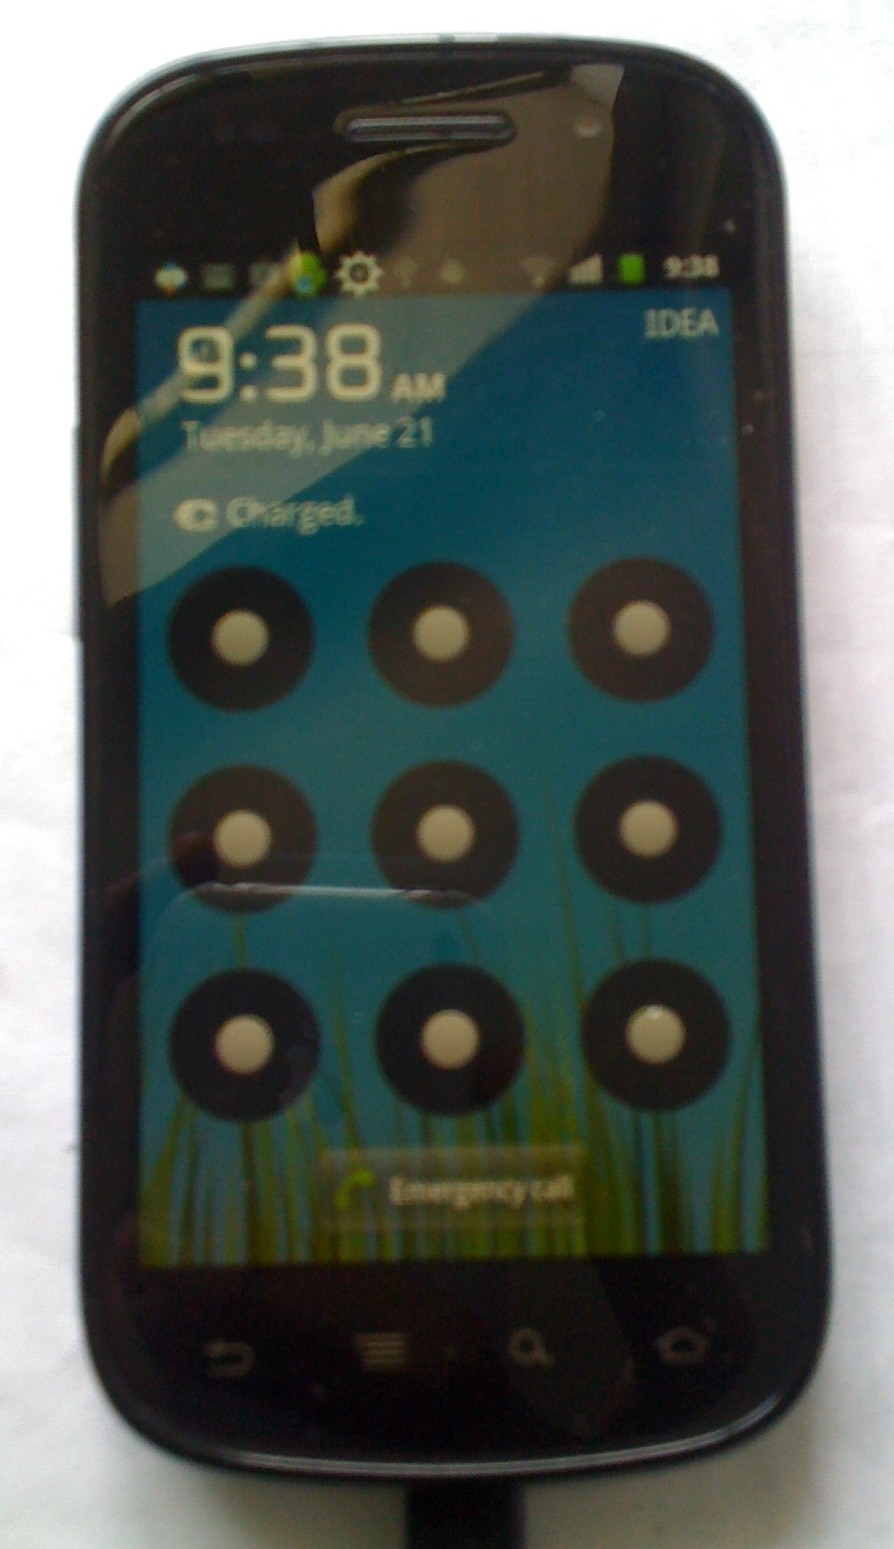
\includegraphics[height=3in]{figures/android_front}
    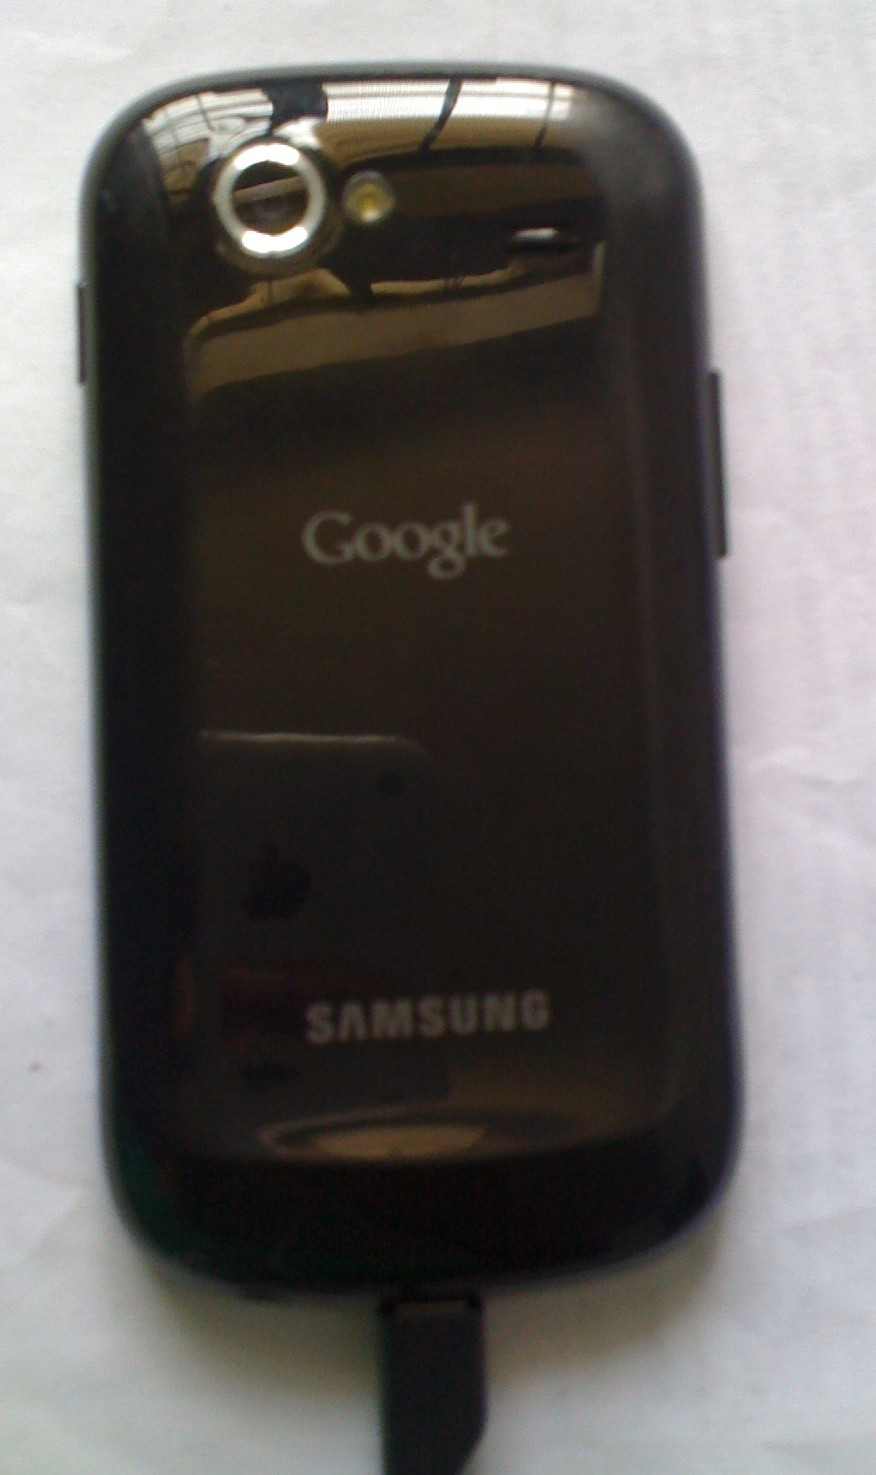
\includegraphics[height=3in]{figures/android_back}
\caption{Google Nexus S manufactured by Samsung}
\end{figure}



\section{Accelerometer}

The MEMS accelerometer on the Nexus S was subject to simple tests to determine 
its noise floor and the degree of separation between signal and noise.
Figure \ref{fig:accel_static} shows a plot of the accelerometer's raw output 
along the Z axis for a stationary device kept on a table. The characteristics
of the accelerometer signal are summarized in Table \ref{tbl:accel_chars}.
As can be clearly observed, the signal degrades while in the palm of a 
user who is standing.

The noise level for the accelerometer was determined to be always less
than $0.6 m/s^2$. The acceleration peaks corresponding to regular walk steps 
usually lie around $2.0 m/s^2$. To allow for a reasonable noise margin and provide
sufficient cushion for additional noise introduced due to the dynamic nature of
walking, we choose a threshold of $1.3 m/s^2$ which is the mean value of the two
peak values. If the absolute value of the Z-axis acceleration sample is less
than this threshold, then the sample will be clamped to zero. For a smartphone
with a similar accelerometer sensor but with different noise characteristics,
the values of the threshold can be varied accordingly. For our purposes, 
the threshold $Q$ is chosen as $1.3 m/s^2$.


\begin{figure}\centering
    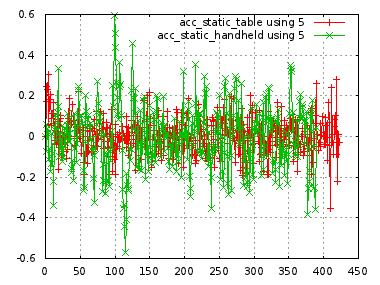
\includegraphics{figures/accel_static.png}
    \caption{Accelerometer Z axis readings when device stationary\label{fig:accel_static}}
\end{figure}

\begin{table}
\centering
\begin{tabular}{c c c c c c c}
\hline
\hline
 & $a_{x,table}$ & $a_{y,table}$ & $a_{z,table}$ & $a_{x,hand-held}$ & $a_{y,hand-held}$ & $a_{z,hand-held}$ \\
\hline
Min & -0.180217 & -0.209914 & -0.352813 & -0.281559 & -0.238432 & \textbf{-0.571722} \\
Median & -0.002995 & 0.001779 & 0.003011 & 0.004029 & -0.005922 & 0.003617 \\
Mean & -0.002065 & -0.002809 & 0.004762 & 0.007291 & -0.003648 & -0.004827 \\
Max & 0.206112 & 0.211490 & 0.306364 & 0.577652 & 0.207061 & \textbf{0.595963} \\
Std. Dev & 0.06985715 & 0.06902411 & 0.08939619 & 0.1100473 & 0.08232208 & \textbf{0.1603238} \\
\hline
\end{tabular}
\caption{Characterization of the Accelerometer (values in $m/s^2$)\label{tbl:accel_chars}}
\end{table}


\section{Magnetometer}

The Nexus S comes with a built in MEMS magnetometer.
It measures the local magnetic field strength in $\mu T$.

In practical tests, the performance is reasonable but the magnetometer has a 
lot of sensor noise and suffers from sensor bias. For example, rotation of 
the smartphone through large angles introduces bias in the readings from the 
magnetometer. Similary, the magnetometer shows a small offset when the device is 
turned through 360 degrees.

Figure \ref{fig:angle_stationary_table}
shows the behaviour of sensor readings under the 2 circumstances when the 
device is on a table and when it is held in the palm of the hand of a user.

\begin{figure}\centering
    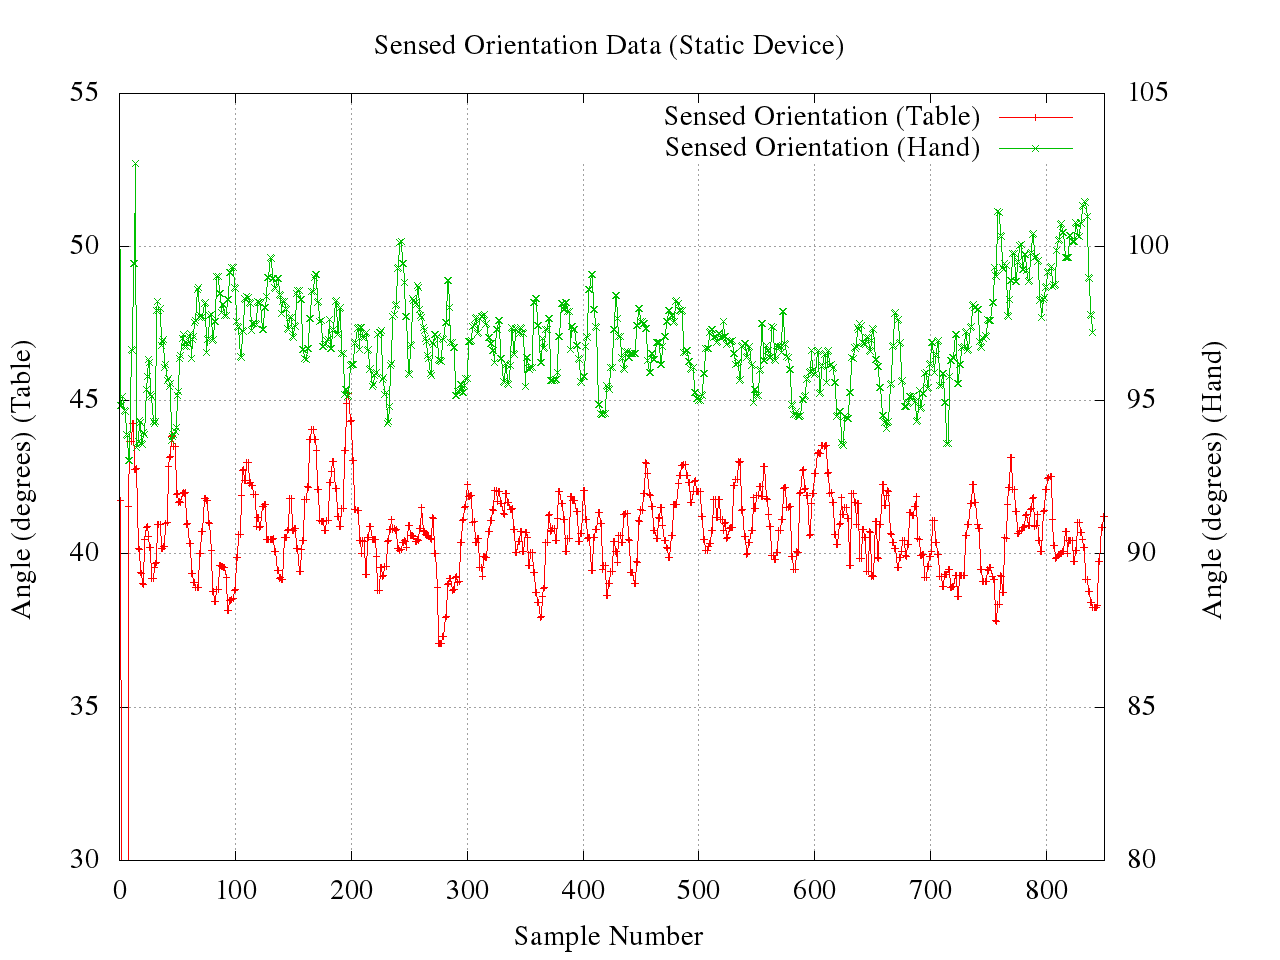
\includegraphics{figures/angle_stationary.png}
    \caption{Derived azimuth angle when smartphone on table\label{fig:angle_stationary_table}}
\end{figure}


\begin{table}
\centering
\begin{tabular}{c c c c}
\hline
\hline
 & $\theta_{table}$ & $\theta_{standing}$ \\
\hline
Maximum Deviation & 8.138436 & 9.688619 \\
Std. Dev. & 1.234318 & 1.521967 \\
\hline
\end{tabular}
\caption{Characteristics of a Stationary Magnetometer (degrees)\label{tbl:angle_chars}}
\end{table}

These values are required to determine choice of parameters for the particle
filter that will be introduced later.

\subsection{Bias study}

Performing rotations in a slow and steady manner yields good results with little
or no bias and sensor lag. See figure \ref{fig:angle_180_rotation_table} which 
shows how the angle measurements behave when the rotated slowly and steadily.
There is only a slight sensor lag and bias visible.

\begin{figure}\centering
    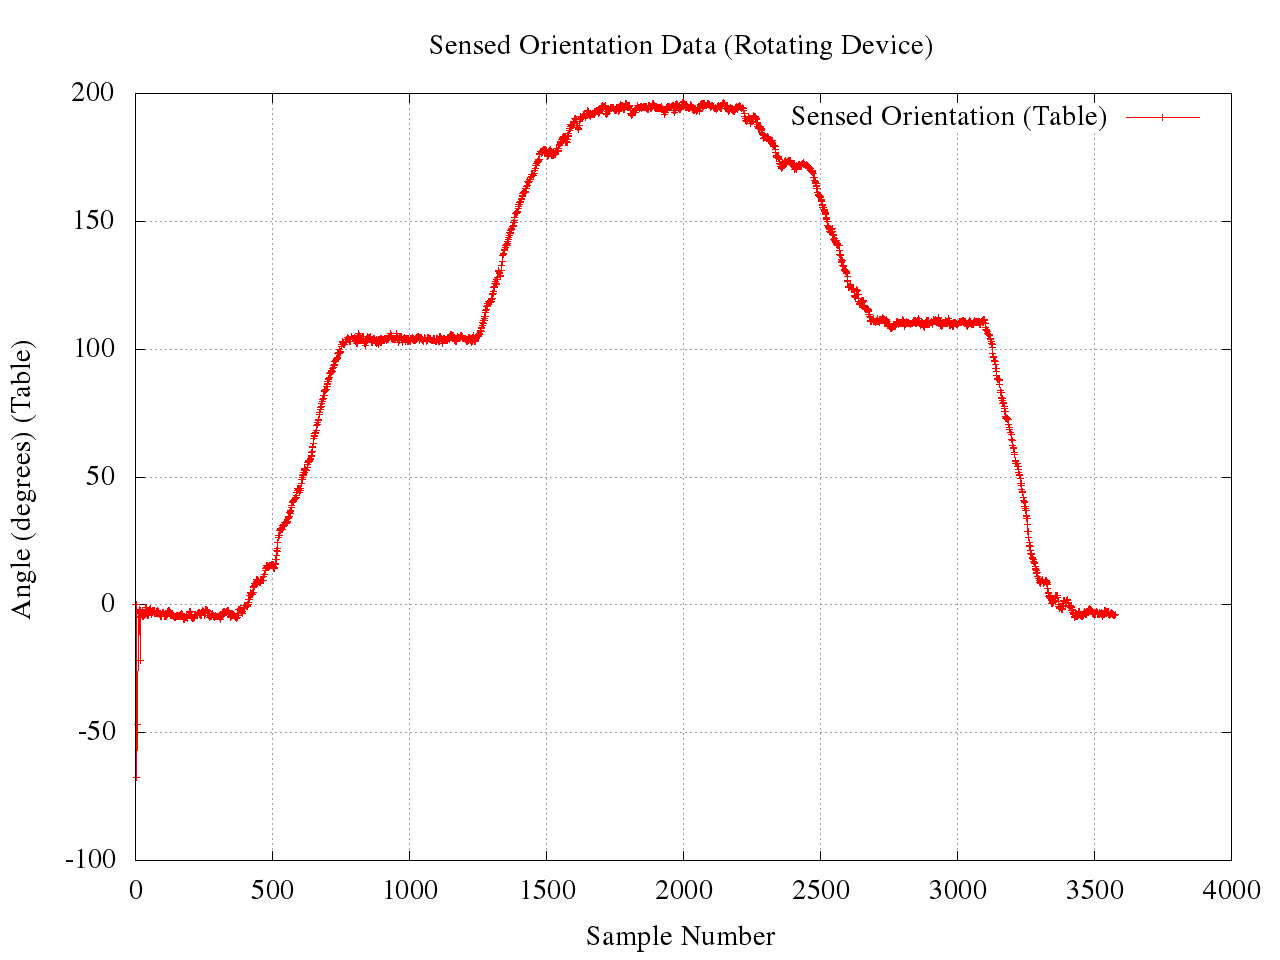
\includegraphics{figures/angle_180_rotation_table.png}
    \caption{Rotation of the phone through 180 degrees (90 degree turns)\label{fig:angle_180_rotation_table}}
\end{figure}


\subsection{Effect of motion}

Although the sensor measurements are stable when the device is on a table,
the measurements go haywire when the device is in a human's hand. See figure
\ref{fig:angle_180_corridoor} - a human is walking along a corridoor and he walks
back. The angle measurements of the return trip are offset by 180 degrees and
the two sets of measurements are compared. You can easily see a large variation
in the angles due to the motion of the human and the dynamic nature of the environment.
Sensor lag and long term sensor value drift is evident in the graph.
This dynamic variation of the measurement of the angle from magnetic north 
introduces error in the inertial navigation system.

\begin{figure}\centering
    \includegraphics{figures/angle_180_corridoor.png}
    \caption{Angle measurements when moving in opp directions.\label{fig:angle_180_corridoor}}
\end{figure}

\begin{table}
\centering
\begin{tabular}{c c c}
\hline
\hline
 & Forward Path & Return Path \\
\hline
Angular Range (Max - Min) & 43.48589 & 32.7897 \\
Standard Deviation & 8.307481 & 5.955799 \\
\hline
\end{tabular}
\caption{Effect of Motion on Orientation Values\label{tbl:angle_motion}}
\end{table}

The values of Table \ref{tbl:angle_motion} indicate the maximum range of 
values over which the angle varies during a walk along a straight corridoor. 
These values are used to set the parameters $\theta_t$ in the algorithm.
The angular range is large but the middle 50\% of the values lie 
between 11 to 13 degrees apart which corresponds with the standard deviation
values measured.

\section{Test Environment\label{sec:test_environment}}

The location chosen for performing all experimental verification of the
proposed work was Floor 3, Wing 7 and 8 of Ravindra Bhawan at the IIT Roorkee
campus. The environment is suitable for this purpose due to a number of reasons:

\begin{enumerate}
\item There are a large number of Wifi Access Points in close proximity 
    installed on the premises.
\item Wifi Access Points of neighbouring wings and floors provide diversity
    to the location fingerprints.
\item Long corridoors of around 30-32 metres each provide long stretches of
    similar environment for evaluation of algorithm performance over larger
    distances.
\end{enumerate}

A map of the location is shown in Figure \ref{fig:ravindra_map}. The red lines
indicate walls, blue lines indicate windows and green lines indicate doors.
Wifi Access Points are marked with stars on the map. This map has been used
for all the experiments detailed below and while determining the results as 
stated in Chapter \ref{chap:results}.

\begin{figure}
    \centering
    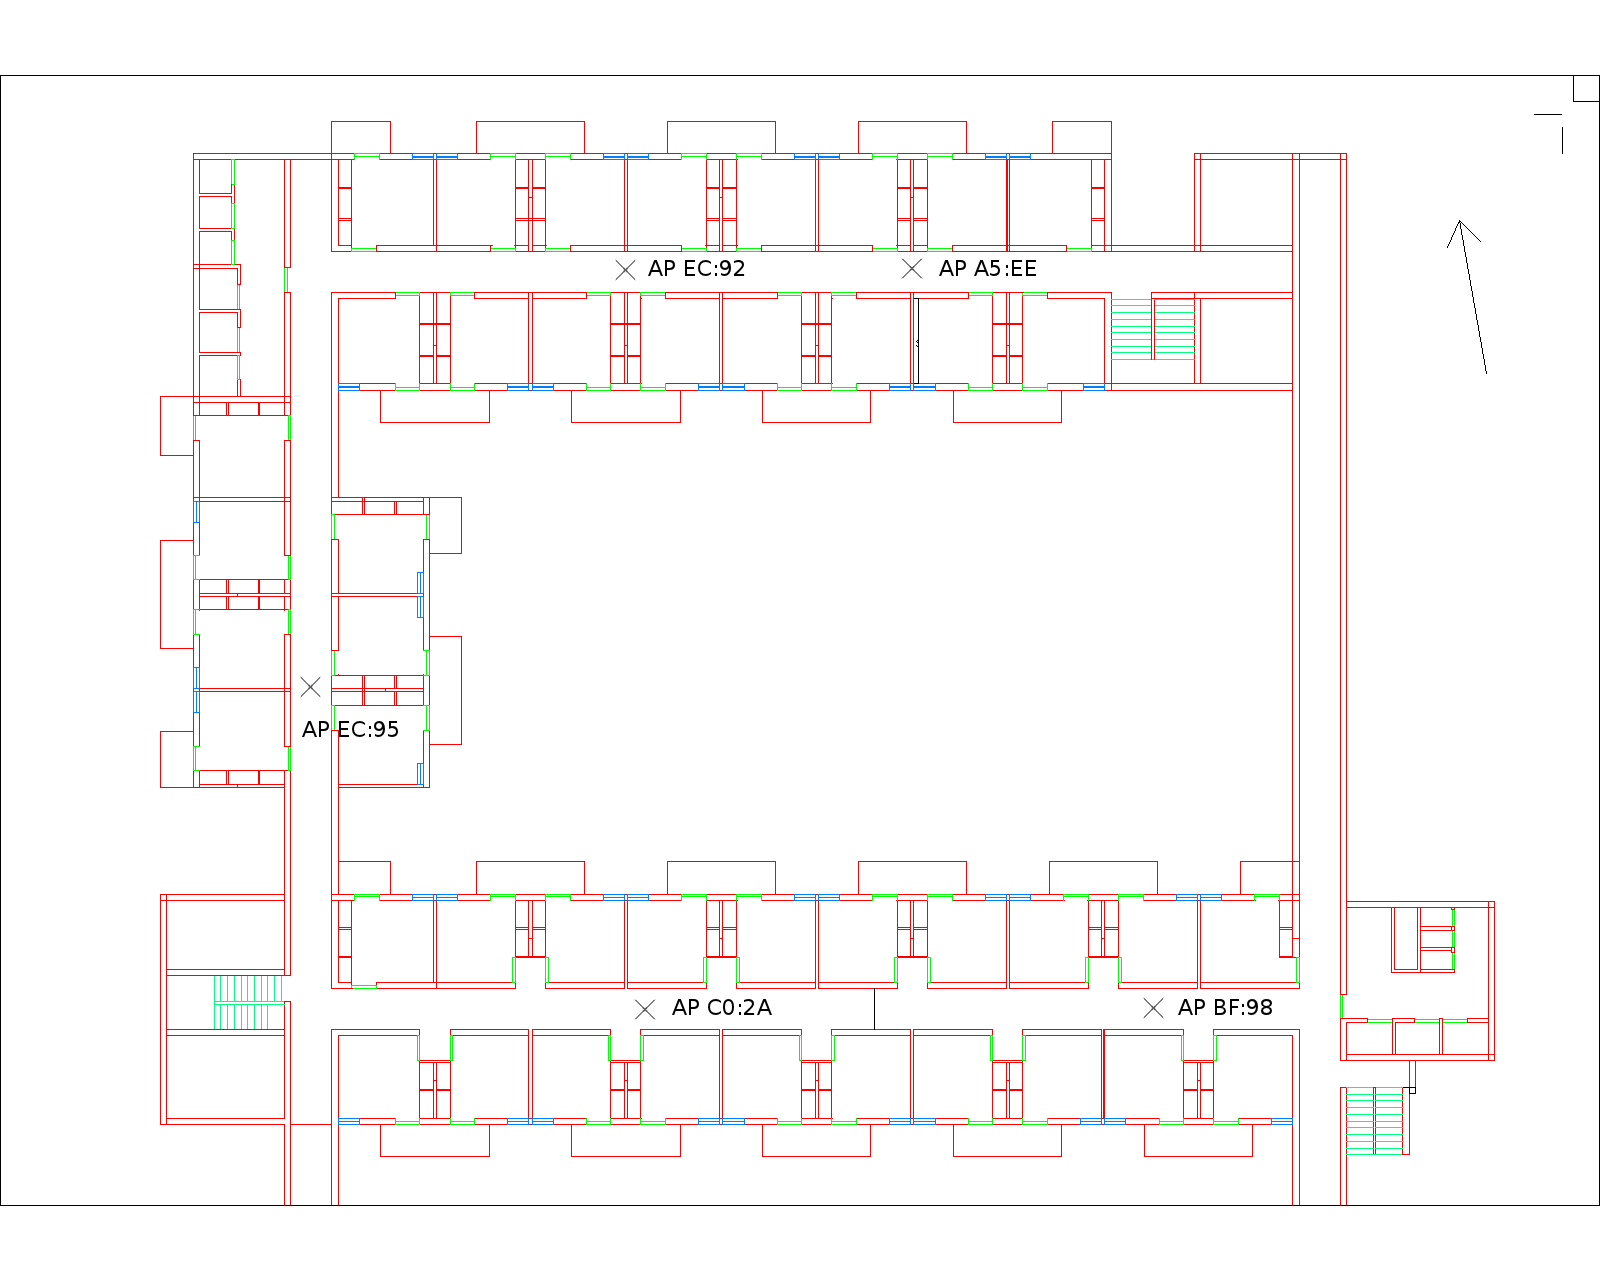
\includegraphics[width=5in]{figures/ravindra_map_ap.png}
    \caption{A map of the experimental environment\label{fig:ravindra_map}}
\end{figure}


\section{Wifi Signal Strength Distribution}

Wifi signals are used in our proposed system during the recovery process.
Other systems and the control algorithms use Wifi for correcting positioning
drift. Hence, it is important to understand the strengths and limitations of 
Wifi based positioning. In order to do so, we need to first characterize
the Wifi signal.

The behaviour of the wifi signal strength distribution for a stationary laptop 
and smartphone was analyzed to characterize the input wifi signal.

\subsubsection{Short term duration}

Figure \ref{fig:closestAPshortterm} shows the variation of signal strength of 
AP EC:95 for a smartphone placed within a room in a 
Non-Line Of Sight configuration.

\begin{figure}\centering
    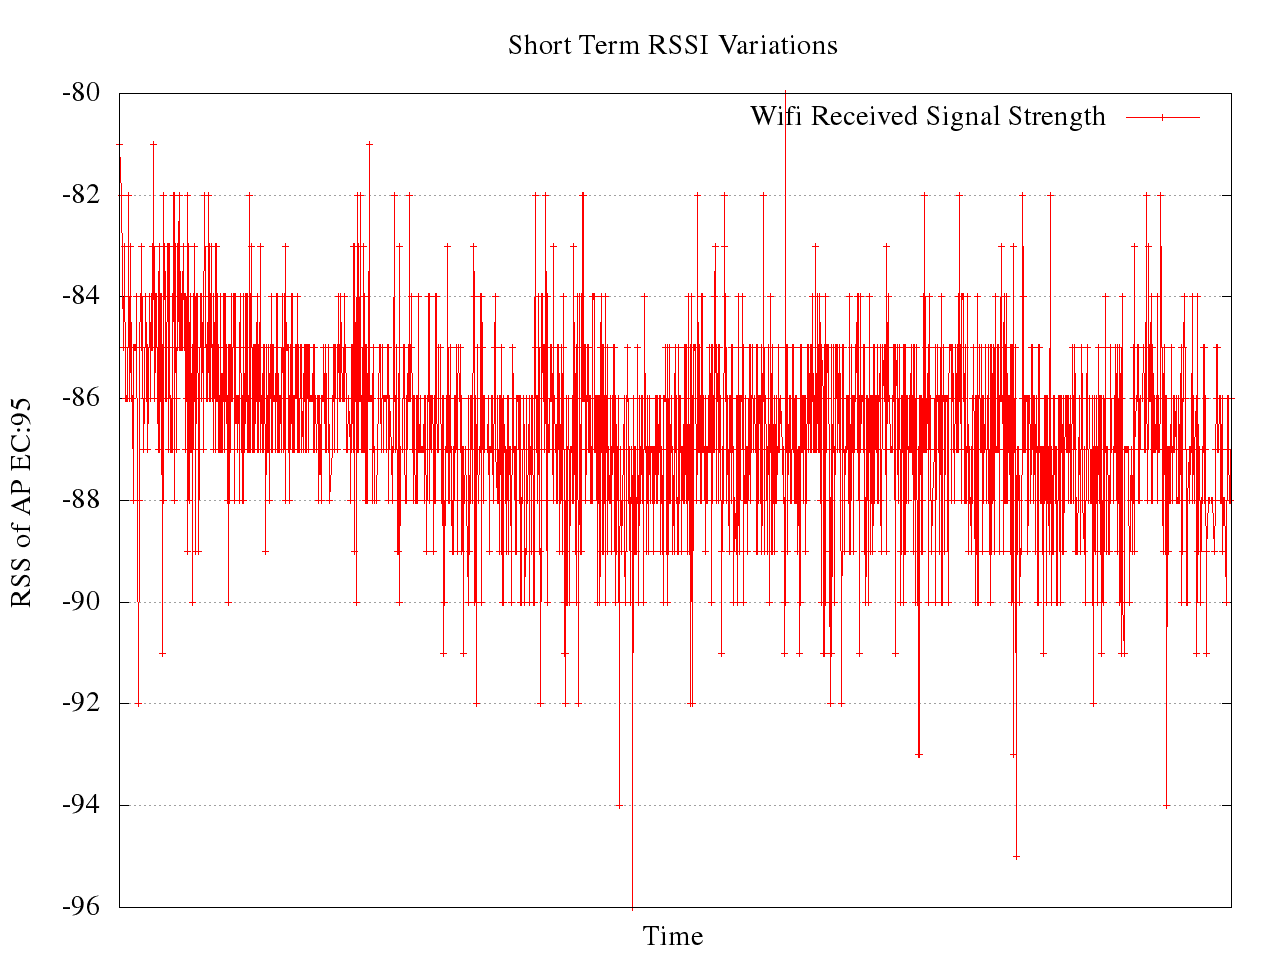
\includegraphics{figures/wifi_short_term.png}
    \caption{Variation of RSSI for AP EC:92 \label{fig:closestAPshortterm}}
\end{figure}

\subsection{7 day study}

The Wifi Access Point RSSI values were monitored over a 7 day period 
(Jan 5 2011 - Jan 13 2011) from room S-152 and the resulting signal strength 
data was analyzed.

\pdfimageresolution 72

\begin{figure}\centering
    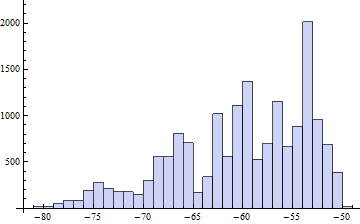
\includegraphics{figures/histogram_00_1C_F0_CB_EC_92.png}
    \caption{Distribution of RSSI values AP EC:92\label{fig:histogram_00_1C_F0_CB_EC_92}}
\end{figure}

As you can see in Figure \ref{fig:histogram_00_1C_F0_CB_EC_92}, the signal 
strength distribution for the closest access point is highly non-gaussian. This
concurs with the conclusions of Kaemarungsi and Krishnamurthy in \cite{KStats}.

\begin{figure}\centering
    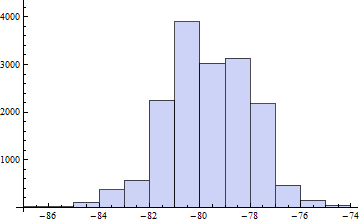
\includegraphics{figures/histogram_00_1C_F0_CB_EC_95.png}
    \caption{Distribution of RSSI values AP EC:95\label{fig:histogram_00_1C_F0_CB_EC_95}}
\end{figure}

\begin{figure}\centering
    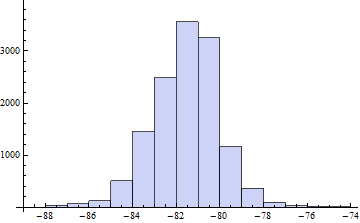
\includegraphics{figures/histogram_00_19_5B_77_A5_EE.png}
    \caption{Distribution of RSSI values for the AP A5:EE\label{fig:histogram_00_19_5B_77_A5_EE}}
\end{figure}

\pdfimageresolution 300

\begin{figure}\centering
    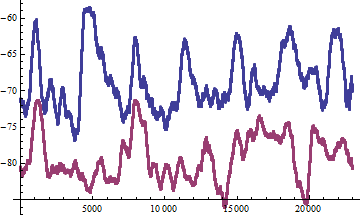
\includegraphics{figures/moving_average.png}
    \caption{3 hour moving average of RSSI values for the 7 day survey\label{fig:moving_average}}
\end{figure}

In contrast, Figure \ref{fig:histogram_00_19_5B_77_A5_EE} doesn't show such a 
pronounced non-gaussian nature whereas 
Figure \ref{fig:histogram_00_1C_F0_CB_EC_95} shows more leanings towards a
non-gaussian distribution.

Table \ref{tbl:wifi_signal_analysis} states the features of the signal with 
respect to 3 different APs. However, this table does not state the entire 
story. 

Figure \ref{fig:moving_average} is the time domain plot of the signal strength
samples smoothed as a moving average over 300 samples as received by a fixed 
location. It is quite evident that the variations in the signal strength 
are highly localized with significant peaks and valleys. Plots for other APs
show this kind of clustering behaviour too but to a lower extent. 
Given the uncorrelated nature of wifi signals, it is highly likely that 
signal variations will not move in a correlated fashion and thus even 
location fingerprinting based systems will find it very difficult to 
create a distance function that will be able to estimate the location of a
device reliably from the RSSI values given that the survey database will 
always be subsampling the signal. 

Thus it is quite evident that the input wifi signal is a highly noisy and
unreliable source of information.


\begin{table}
\centering
\begin{tabular}{c c c c c c c c c}
\hline
\hline
 & Min & $1^{st}$ quartile & Median & Mean & $3^{rd}$ quartile & Max & NA & SD\\
\hline
AP EC:92 & -82.00 & -66.00 & -60.00 & -60.62 & -55.00 & -49.00 & 27.36\% & 6.638592\\
AP EC:95 & -87.00 & -81.00 & -80.00 & -80.16 & -79.00 & -74.00 & 30.64\% & 1.691343\\
AP A5:EE & -89.00 & -83.00 & -82.00 & -82.05 & -81.00 & -73.00 & 43.48\% & 1.580761\\
\hline
\end{tabular}
\caption{Wifi Signal Analysis\label{tbl:wifi_signal_analysis}}
\end{table}

\section{Effect of motion on signal strengths}

To analyze the effect of motion on the RSSI values from the APs, a simple walking
test was done along a corridoor. The variation of RSSI values seen from the AP in
the corridoor is shown in \ref{fig:wifi_corridoor_walk}.

\begin{figure}\centering
    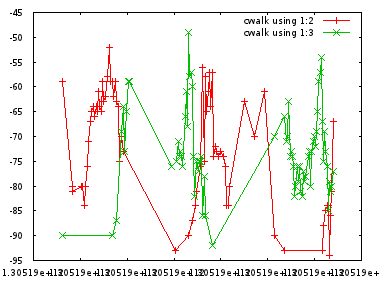
\includegraphics{figures/wifi_corridoor_walk.png}
    \caption{AP EC:95 RSSI: Walk up and down the corridoor\label{fig:wifi_corridoor_walk}}
\end{figure}


\subsection{Inferences}
From the figure, it can be clearly seen that orientation with respect to 
AP is important. There is significant noise in the signal even though the AP 
is in the line of sight. Thus retaining orientation data with respect to 
an AP is an important criteria while surveying the test environment to 
collect location fingerprints.

\section{Generating a Location Fingerprinting Dataset}

A Wifi Survey was carried out in the test environment to generate a location 
fingerprint dataset. To ensure uniform sampling of the environment, 
a $1m \times 1m$ grid was set up on the ground and Wifi RSSI readings were taken 
at 8 different orientations per point on the floor. 
Figure \ref{fig:grid_pic} shows a snapshot of a small area of the test environment.
Grid points have been marked out on the floor. 
Wifi RSSI samples were taken at these grid points along 8 different orientation 
values. Some samples, however, could not be taken due to obstructions 
present at the site.

\begin{figure}
    \centering
    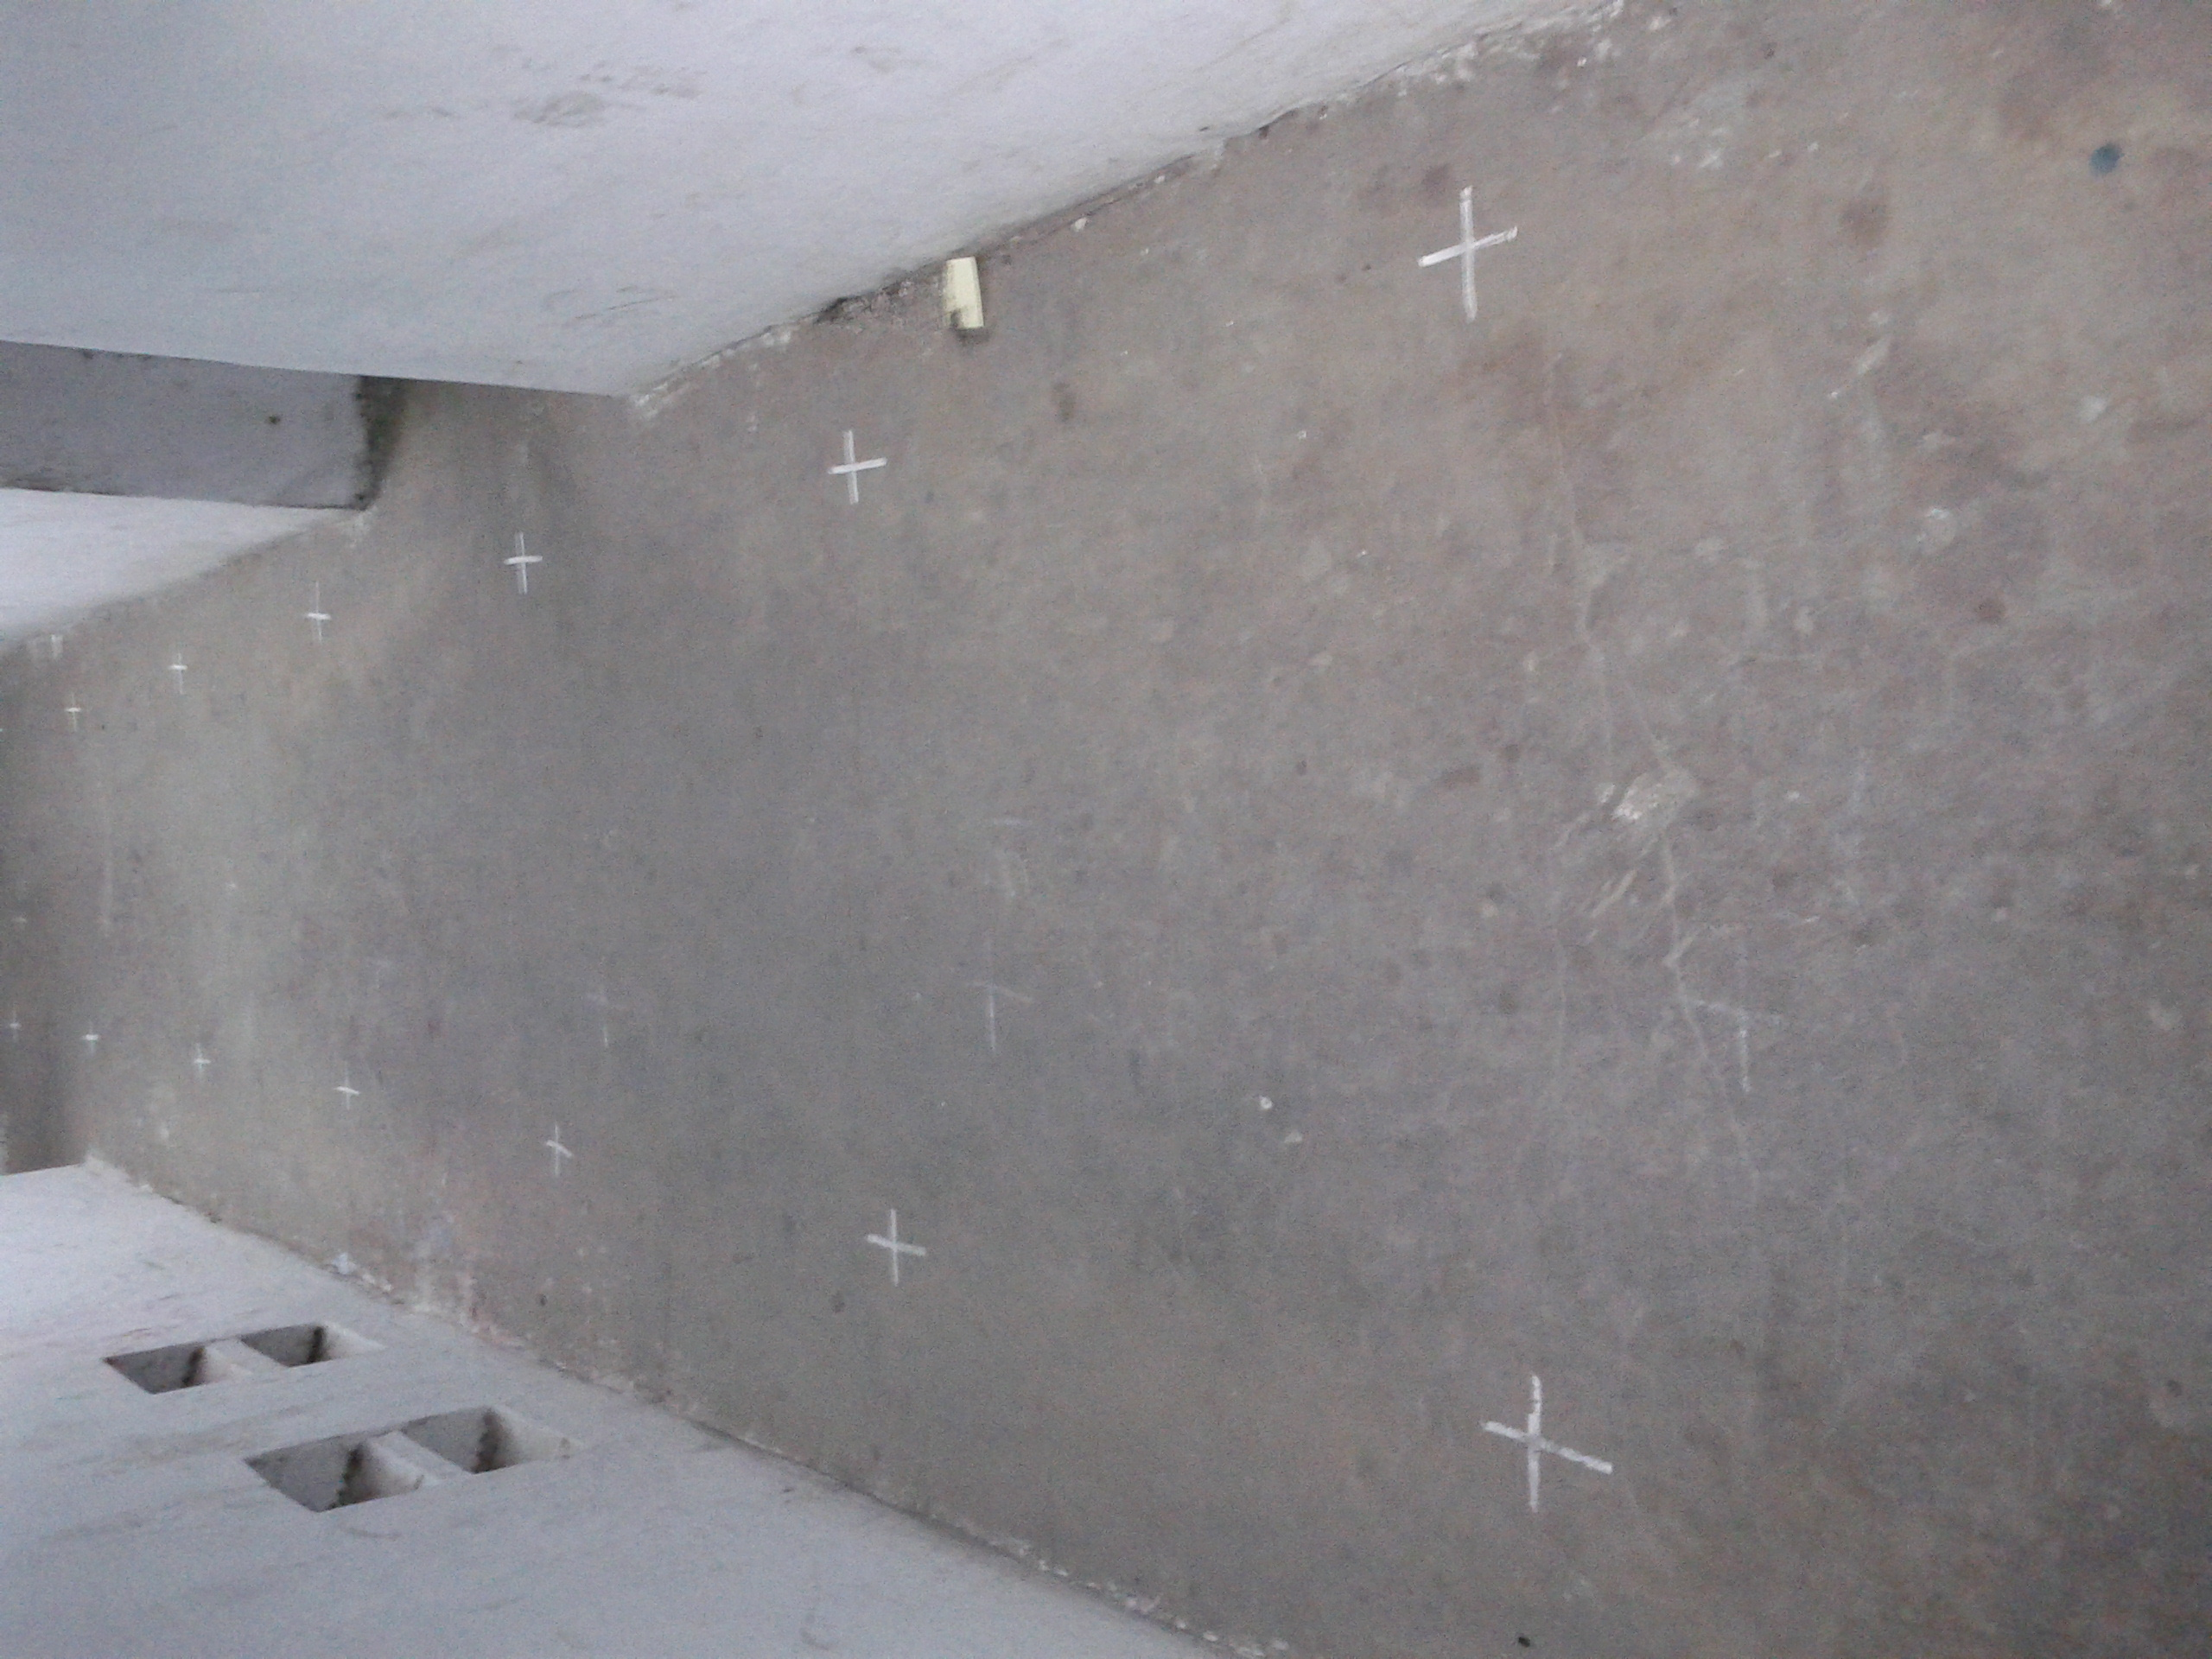
\includegraphics[width=5in,angle=270]{figures/grid_pic}
    \caption{Picture of the $1m \times 1m$ grid drawn on the floor\label{fig:grid_pic}}
\end{figure}

\section{Testing Wifi Positioning Accuracy using KNN\label{sec:knn_pos}}

A KNN based location system was implemented to test location accuracy for positioning using Wifi Signal Strengths. 
This was work done as part of the Masters project in the same test location. 
The results of the project are included here. Although the project was 
done using a laptop instead of a smartphone and with a different set of survey data, 
it is expected that the results will be comparable as the test environment was the same.

\begin{table}[h]
    \centering
    \caption{Performance of KNN based indoor positioning system \label{tab:knnperf}}
    \begin{tabular}{|l|c|c|c|}
    \hline
              & Mean Error $\bar{e}$ (m) & $\sigma_{error}$ (m) & $\bar{e} + 2 \sigma_{error}$ \\
    \hline
    \hline
    $K = 1$    & 2.8 & 2.7 & 8.2 \\
    $K = 2$    & 2.8 & 2.7 & 8.2 \\
    $K = 3$    & 2.7 & 2.7 & 8.1 \\
    $K = 4$    & 2.3 & 2.8 & 7.9 \\
    \hline
    \end{tabular}

\end{table}

\section{Summary}

To conclude, we can state that by doing all the experiments and other 
ground-work mentioned in this chapter, we have obtained a fair idea 
about the inputs of the system and various system parameters required
for the algorithms. The groundwork thus helps in guiding the implementation of
the system. Since groundwork was being done in conjunction with algorithm
design, some feedback from the groundwork was also incorporated into improving
the design of the proposed method of Chapter \ref{chap:proposed_method}.

By doing the groundwork, we have been able to derive the ranges of parameters of 
the proposed algorithm. These ranges are listed in Table \ref{tbl:algo_params}.

\begin{table}
\centering
\begin{tabular}{c c}
\hline
\hline
Parameter & Value\\
\hline
For Noise Filtering & \\
Threshold $T$ & $> 0.352813$\\
Threshold $Q$ & $Q > 0.595963$ and $Q < 2.0$\\
\hline
For Orientation Bias & \\
$\sigma_{angle}$ & 8.307481 degrees\\
\hline
For NN based positioning & \\
Wifi Orientation Tolerance & $> 43.48589$ degrees\\
Wifi Positioning Error & $> 2.8 m$ with S.D. $> 2.7 m$\\
\hline
\end{tabular}
\caption{Algorithm Parameters Determined by Ground Work\label{tbl:algo_params}}
\end{table}


\chapter{Implementation Details\label{chap:implementation_details}}

\section{Background on Android Application Development}

\subsection{The Android OS}

The Android OS was initiated as an open source project by Google  
to make application development easier for mobile devices. In order to 
do so, Google engineers created a customized Java Virtual Machine 
(called Dalvik VM) with resource saving features 
to make running Java applications on embedded devices feasible.
A large section of the Java Standard Library was then bolted onto the 
JVM by leveraging the open source Apache Harmony project.\todo{cite both} 
The typical structure of an Android Application built on the Android OS 
is shown in Figure \ref{fig:Android_OS_Structure}.

\begin{figure}
\centering
\begin{picture}(300,300)
%\graphpaper(0,0)(300,300)
\put(0,0){\framebox(300,30){Device Hardware}}
\put(0,50){\framebox(300,30){Android OS}}
\put(0,100){\framebox(80,30){Android App}}\put(110,100){\framebox(80,30){Android App}}\put(220,100){\framebox(80,30){Android App}}
\put(40,100){\vector(0,-1){20}}\put(150,100){\vector(0,-1){20}}\put(260,100){\vector(0,-1){20}}
\end{picture}
\caption{Typical Structure of Android OS\label{fig:Android_OS_Structure}}
\end{figure}

\section{Application Development Tools}

Applications for Android are usually written in Java and are run on the 
custom Dalvik VM. Embedded programming is usually difficult because of 
limited visibility of the way the code runs on the target device (a smartphone).
To make development of apps for Android easier, custom tooling for Android 
has been developed that integrates with the Eclipse IDE toolchain.
The tools help to
interface with a development smartphone running an Android OS. They provide a
direct install-uninstall mechanism for applications under development 
and they also provide a debug bridge - called the ADB through which 
the Application code running on the smartphone may be debugged via debugging
tools on the host computer. A logging mechanism is also provided wherein 
application logs running on the device may be made visible in realtime 
on the host computer through the ADB. These tools go a long way in making 
development easier and help the programmer detect root causes of bugs faster.


\section{The Android Application Lifecycle\label{sec:android_lifecycle}}

Android applications are very different from the normal system executables
that we are used to programming. Executables once launched have complete 
system control during execution. They demand resources and release them at 
will depending on how they have been programmed. They are pre-empted and 
resumed transparently by the Kernel scheduler. However, such a mode of
execution is unsuitable for applications built for the mobile device. 
These applications need to be aware of their internal state at all times.
The user may pre-empt any application at any time and the system may 
suspend or even kill applications without warning to reclaim resources.
Applications are therefore expected to be written to follow an event machine 
lifecycle and are expected to save their state whenever they get pre-empted. 
The lifecycle of a typical Android application is shown in 
Figure \ref{fig:android_lifecycle}.


\begin{figure}
\caption{Android Application Lifecycle (Simplified)\label{fig:android_lifecycle}}
\end{figure}

The application typically starts off the 'Created' state, progresses 
to the 'Resumed' state. It may oscillate between the 'Resumed' and 'Paused' states
several times during the course of the execution lifetime of the application 
and then it finally transitions to the 'Finished' state when it is killed by 
the system either automatically or in response to a user action. All 
processing in the application is done either in response to a User action, 
a state change in the application lifecycle or in response to System 
messages delivered asynchronously to the application via \emph{BroadcastReceivers} 
or \emph{Intents}. (\emph{BroadcastReceiver} and \emph{Intent} are important
classes in the Android framework).

\section{System Architecture}

As is clear from the previous section, the Android OS expects applications to 
be event-driven. In our case, events are being generated by the user 
not through direct interaction with the application via the UI but through 
indirect interaction via the sensors onboard the device. This naturally 
leads to a bottom-up design of the system on the lines similar to protocol
stacks seen commonly in the case of Computer Networks. The analogy
being drawn here is that a packet receive event in the case of a 
protocol stack is similar to a sensor event generated for our system. 

The complete layered structure of the application is shown in Figure 
\ref{fig:system_architecture}. 

\begin{figure}
    \centering
    \includegraphics{figures/system_architecture}
    \caption{System Architecture\label{fig:system_architecture}}
\end{figure}

At the lowest layer, we have the \textbf{Sensor Unification Layer}. This layer is 
important as the Android API separates the event delivery mechanism 
for a Wifi SCAN event and the event delivery mechanism for a sensor 
sample event. The rationale behind this being that sensors are passive 
environment samplers while the Wifi NIC is an active communication 
device and is not typically intended to be used as a sensor. The \textbf{Sensor 
Unification Layer} works very hard to unify Wifi SCAN event results and 
sensor sample results into a single uniform events system to which 
a higher layer can subscribe by registering a callback object. Whenever 
a sensor event takes place for which higher layers have requested notification,
all registered callbacks for that event are executed by this layer. Thus,
higher layers can request access to sensor events by just registering an 
appropriate callback with this layer. The unification layer takes care of 
interfacing with the Android SensorManager API and the Android WifiManager API
and exposes lifecycle methods - \tt{pause} and \tt{resume} which free up 
higher layers from performing appropriate registrations and de-registrations
of sensor event handlers when they intend to go to sleep. The class that 
provides the API for the higher layers is the \emph{SensorLifecycleManager} class
and the critical class for implementation of this layer is the 
\emph{HWSensorEventListener} and \emph{WifiScanEventListener} classes. 






The problem being implemented has a natural event-driven layered structure. 
We are taking
low level sensor events being generated at a fast pace and converting 
them to "step" events that take place much more rarely. These step events 
are then processed 

\section{System Implementation of the Lifecycle}

The Android Application Lifecycle referred in Section \ref{sec:android_lifecycle}
primarily deals with high level user actions such as going idle, switching 
off the screen, exiting the application etc. 

\missingfigure{Architecture of system}

\missingfigure{List of major classes}

\missingfigure{Their interactions}


\chapter{Experiments and Results\label{chap:results}}

All the experiments and results of this Chapter are performed in the 
same test environment as described in Section \ref{sec:test_environment} 
using the Android Application implementation described in Chapter 
\ref{chap:implementation_details}.
Based on the groundwork performed, the parameters of the algorithms were chosen.
This chapter discusses the performance of the proposed approach and the 
two control algorithms based on the same set of selected parameters as the 
proposed algorithm.

%\subsection{Acceleration}

%Raw acceleration information is available on the Android device via samples 
%from a 3 axis MEMS accelerometer. The device reports the sensor as 
%a ``KR3DM 3-axis Accelerometer"\todo{Cite datasheet}. Thus acceleration values along all 3 axes
%are available.

%\subsection{Magnetic Field}

%Magnetic field information is available on the Android device via samples 
%from a 3 axis magnetometer. The device reports the device as an
%``AK8973 3-axis Magnetic field sensor".\todo{Cite datasheet}

%\subsection{Cameras}

%A 5 megapixel camera is present rear-facing on the Nexus S. A 0.6 megapixel
%front facing camera is also present on the device.\todo{Cite datasheet or official specs}

%\subsection{Wifi Receiver}

%A standard 802.11 b/g/n capable Wireless NIC is present on the device. Thus,
%it is compatible with both 2.4 GHz and 5 GHz frequency band IEEE 802.11 networks.

%\subsection{Additional Inputs}

%\subsubsection{Map Information}

%A blueprint of the test area was converted into a digital map using AutoCAD
%and the resulting map was exported as a high resolution image ($1600px \times 1280px$)
%and a low resolution version ($640px \times 480px$). Due to memory constraints, 
%the low resolution version of the map will be used for providing map information
%to the algorithm as it expands out to only 1.2MB in uncompressed form as 
%compared to 8.19MB for the higher resolution one. The additional memory 
%usage is significant as the Android OS severely limits the heap limits of 
%single applications. For some mobile devices, the heap limit is as low as
%16 MB.

%\subsubsection{Wifi Site Survey Information}

%It is possible to do a site survey of the test area to generate a database of
%Wifi fingerprints which may be used for implementing Wifi based positioning
%and tracking algorithms.


\section{The Filtering Algorithm}

The threshold ($Q$) for the filtering algorithm described in Section 
\ref{sec:NoiseClamping} was chosen as the mean of the 
ranges determined in the groundwork to provide adequate noise margin. 
Therefore, the threshold for the noise filter was set at $1.3 m/s^2$.

The clamping technique described in Section \ref{sec:NoiseClamping} was employed
to filter the raw acceleration.

The effect of the clamping on the raw accelerometer data is shown in 
Figure \ref{fig:accel_raw}. Figure \ref{fig:accel_diff} shows the sensor noise
that is rejected around zero enabling clean detection of peaks corresponding to
the steps.

\begin{figure}[tbph]
    \centering
    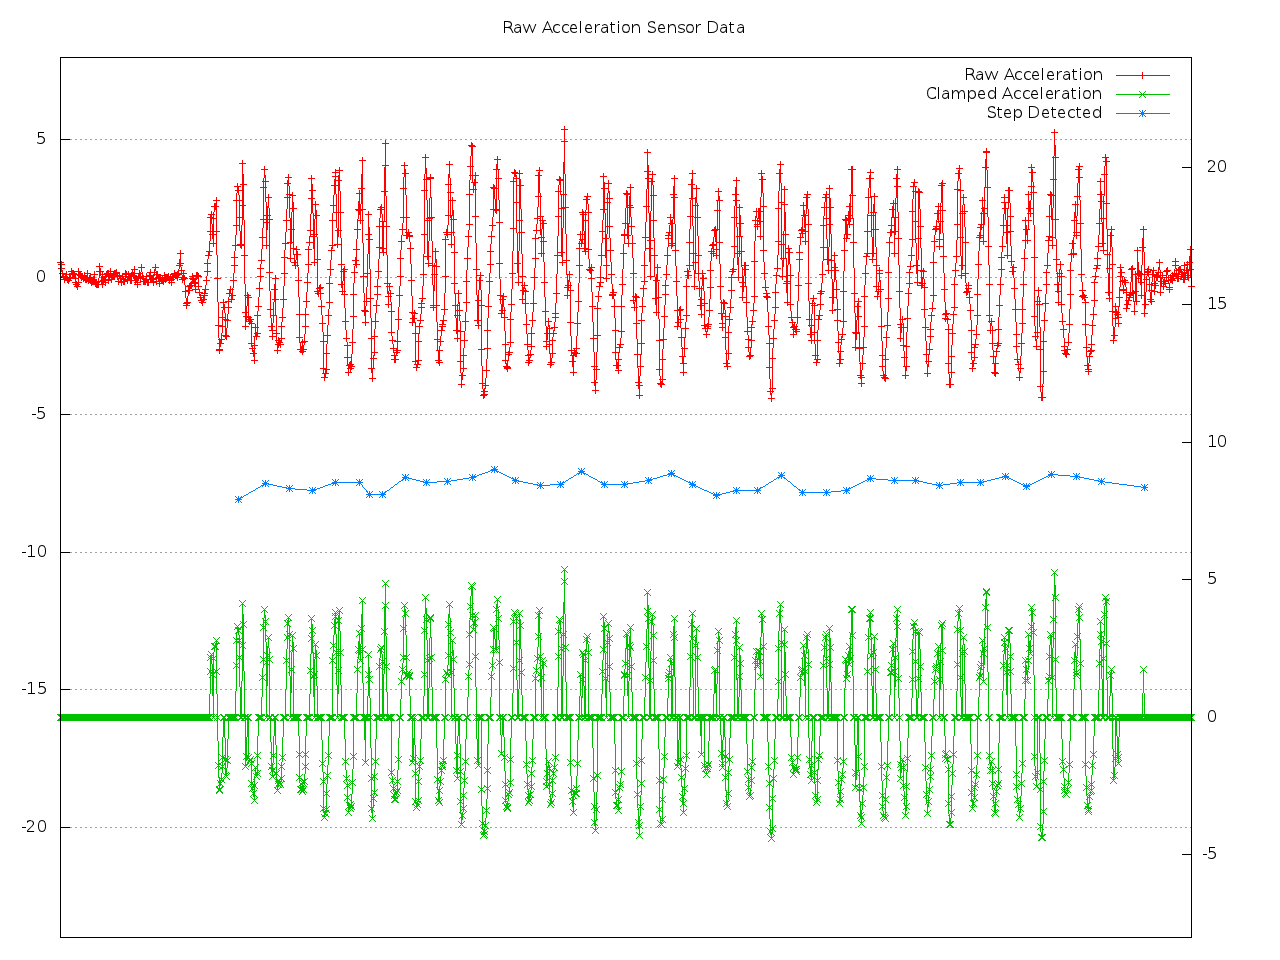
\includegraphics{figures/accel_raw.png}
    \caption{Output of the Filtering algorithm \label{fig:accel_raw}}
\end{figure}

\begin{figure}[tbph]
    \centering
    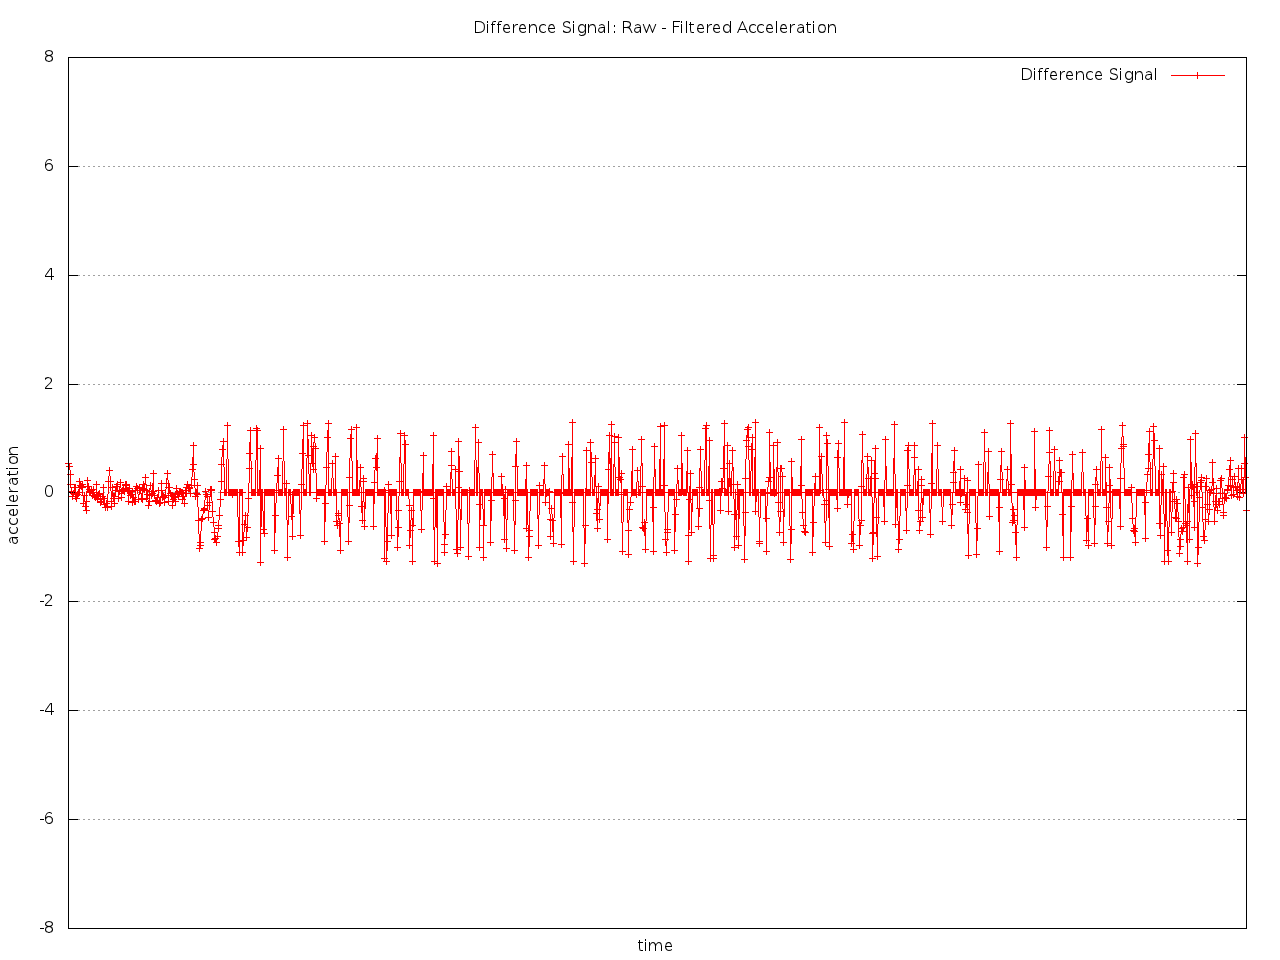
\includegraphics{figures/accel_diff.png}
    \caption{Rejected signal from the Accelerometer sensor \label{fig:accel_diff}}
\end{figure}


\section{Step detection procedure}

The step detection procedures of Section \ref{sec:step_detection} were analyzed
using sensor data of the accelerometer on the Android mobile phone. 
The simple zero crossing method on unfiltered data was used as a control 
algorithm to estimate the improvement in step detection.

The comparative graph of the performance of the step detection procedures 
is shown in Figure \ref{fig:csteps}. Table \ref{tbl:step_table} shows how the 
methods performed in relation with the actual number of steps detected.


\begin{table}[tbph]
\centering
\begin{tabular}{||l|c||}
\hline
\hline
\textbf{Algorithm} & \textbf{Steps Detected} \\
\hline
Simple Zero Crossings Count & 109 \\
Zero Crossings on Filtered Data & 41 \\
Peaks and Valley Method & 41 \\
\textbf{Actual Number of Steps} & \textbf{40} \\
\hline
\hline
\end{tabular}
\caption{Step Detection Performance\label{tbl:step_table}}
\end{table}

It can be seen that a simple Zero Crossing method performs similarly to the 
Peaks and Valley method. From the time based graph plotted in 
Figure \ref{fig:csteps}, it can be seen that the Peaks and Valley method 
slightly lags the Zero Crossing method in time. This is to be expected as this
method detects a step only when the next peak is detected and thus suffers a 
lag of about half a step.

\begin{figure}[tbph]
    \centering
    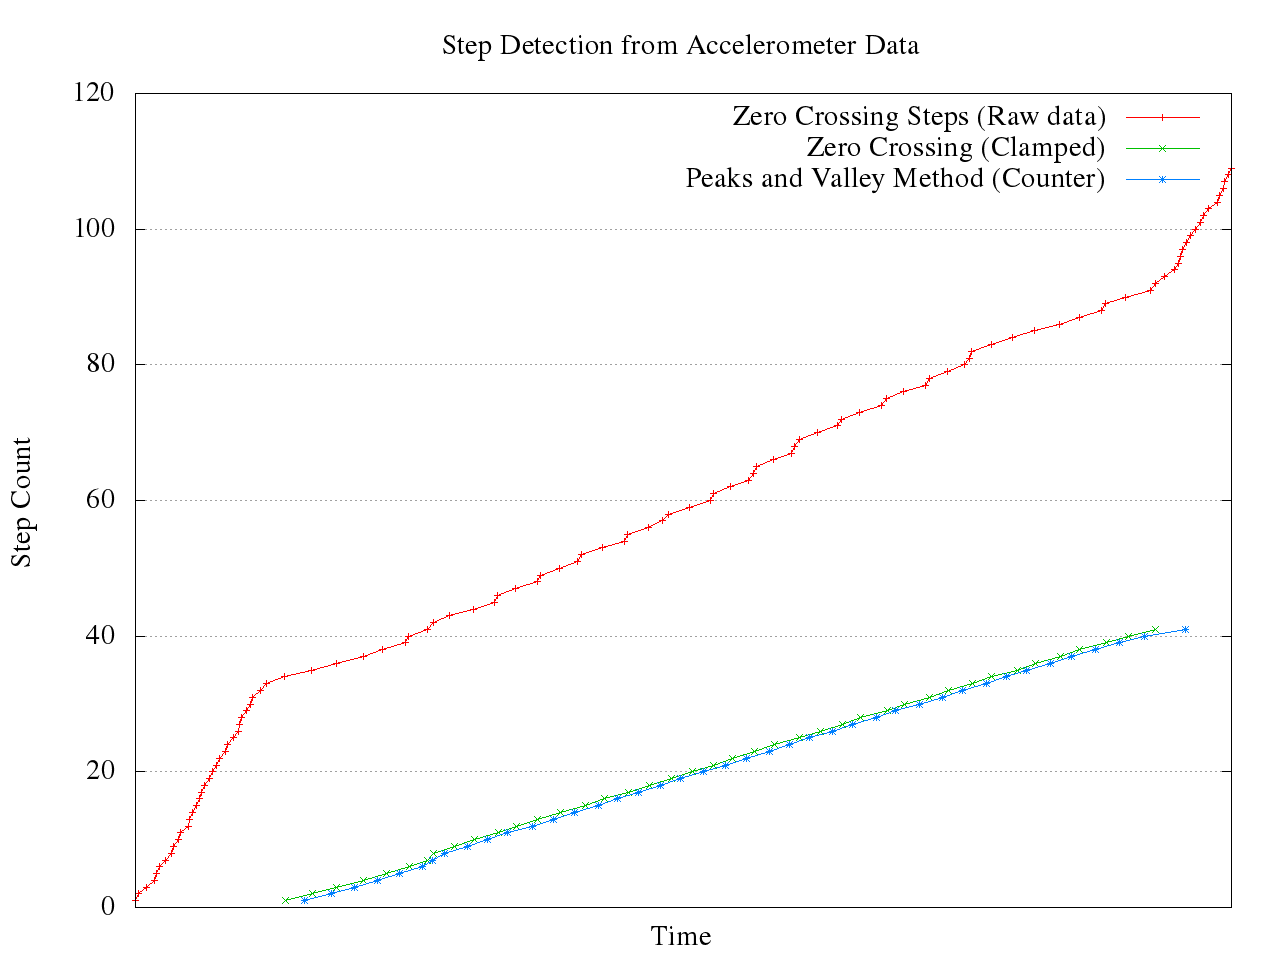
\includegraphics{figures/csteps.png}
    \caption{Performance of Step Detection Algorithms\label{fig:csteps}}
\end{figure}


\section{First Fix}

This section analyzes the two different methods of \ref{sec:first_fix}
used for obtaining the first fix for the algorithm. 

\subsection{Experimental setup}

All the experments were performed with the same Android device (the Samsung 
Nexus S) and with the same application software. Users were familiar with 
touch screen phones and were well aware of the layout of the building. None of
the users had had any prior exposure to the map of the building and did not 
know the direction of True North. Details of the experiments performed 
are specified in Sections \ref{sec:direct_selection} and \ref{sec:qrcode_selection}

\subsection{Direct Selection of Location on a Map\label{sec:direct_selection}}

Five test subjects were asked to mark out their current position on a
map by simply touching the corresponding location on the map shown on the 
touchscreen of the device. The map was shown at a fixed resolution to all 
test subjects in order to make their responses comparable. Their positions 
on the touchscreen were snapped to the nearest 1 m grid pixel for ease of use.

The test were also allowed to retry locating themselves on the map in case they
were not satisfied with their initial results. All their location attempts were
logged for later analysis.The following facts were observed during the process of 
selection:

\begin{enumerate}
\item Some users had an initial difficulty in orienting themselves with regard to 
    the map supplied.
\item As the map contained blocks of rooms that were similar looking,
    initial errors were made in orientation. However, they attempted to 
    correct their errors when the mistake was realized.
\item Some users felt extremely frustrated by the direct selection procedure
    primarily because they could not mark out their locations precisely due
    to the large surface area of contact of their fingers with the touch
    screen. The variability of selection of the contact point while using 
    the touchscreen contributed to an increase in the number of attempts
    required to correctly mark their positions on the map.
\end{enumerate}

\begin{table}
\centering
\begin{tabular}{p{0.8in} p{0.8in} p{3.4in}}
\hline
\hline
User     & Retries & Comments \\
\hline
1               & 6                  & This user had difficulty orienting himself with respect to the map. \\
2               & 0                  & -- \\
3               & 2                  & -- \\
4               & 2                  & -- \\
5               & 15                 & This user had difficulty with the touchscreen contact areas. He was not a user of a touch screen phone. He also had an initial difficulty with orientating himself on the map. \\
\hline
\end{tabular}
\caption{Number of Retries for a Satisfactory First Fix\label{tbl:num_loc_attempts}}
\end{table}

\subsection{QRCode Based Selection of Location\label{sec:qrcode_selection}}

To evaluate the efficiency of determining first fix via QRCodes in comparison 
to the direct location selection method, an experiment was set up. 
The experiment was performed in conjunction with the experment of 
Section \ref{sec:direct_selection}, users were asked to locate themselves
by snapping a QRCode pasted on the wall instead of marking their starting 
location on a map.

The users were then positioned at various distances from the QRCode and 
asked whether they would make the effort to go to the QRCode to snap their
starting location while using the application or whether they would prefer
the manual method.

The following observations were made regarding the QRCode method for first
fix:

\begin{enumerate}
\item QRCode selection via the camera was a fast process, usually not requiring
    more than 10 seconds on behalf of the user.
\item Users were consistently located at distances less than 1 meter from 
    the QRCode. In most cases, the users were at a distance of around 30 cm 
    from the QRCode pasted on the wall. 
\item There was an instance where poor lighting delayed the capture of the
    QRCode and the QRCode could be successfully captured only after a 
    fluorescent tubelight was switched on to provide adequate lighting.
\end{enumerate}

\subsection{Comparison between the two methods}

After processing the results of the experiments, it was determined that 
users overwhelmingly preferred the QRCode method for first fix acquisition.
They were willing to walk up to $5 m$ to the nearest QRCoded location in 
order to take advantage of the facility. The results of the comparative 
survey are listed in Table \ref{tbl:QRCode_comparison_survey}.

\begin{table}
\centering
\begin{tabular}{p{0.8in} p{0.8in} p{0.8in} p{0.8in}}
\hline
\hline
User Number & First fix by manual method (Ease of use: scale of 5) & First fix by QRCodes (Ease of use: scale of 5) & Building familiarity required for manual method (scale of 5) \\
\hline 
1 & 1 & 5 & 5 \\
2 & 2 & 3 & 4 \\ 
3 & 2 & 4 & 5 \\
4 & 3 & 5 & 4 \\
5 & 1 & 5 & 4 \\
\hline
{\bf Mean} & {\bf 1.8} & {\bf 4.4} & {\bf 4.4} \\
\hline
\end{tabular}
\caption{Comparison of QRCode based first fix with the Manual Marking Method\label{tbl:QRCode_comparison_survey}}
\end{table}

\subsection{User Feedback}

Users in their comments indicated that potential improvements to the 
application were possible. For example, if the application could determine 
roughly their current location and then provide just that subset of the map
in which the user was located, the speed of providing the first fix location 
by a manual method could be improved.

\section{Determining the Training Constant}

In a separate experiment, three test subjects were asked to walk between 
2 QRCoded locations. The first fix was taken using the QRCode method and 
the training constant was thus estimated based on the number of steps 
detected and the known distance between the 2 QRCoded locations.

The locations used for this test were along a corridoor and were about $30 m$
apart. The tests were repeated thrice for each subject. The step constants
for the users were different but consistent.

\section{Step variation analysis}

To see the performance of the algorithm to step variations, an experiment 
was performed wherein a test subject walked at three distinct speeds
along a straight corridoor. The subject paused for a short while between 
the three distinct segments to maintain separation of speeds.

The three segments of the walk had the following
characteristics:

\begin{enumerate}
\item The test subject walked with very light steps, almost shuffling along. 
\item The test subject walked with regular steps along the corridoor.
\item The test subject walked with large steps along the corridoor in a motion
    that approximated running.
\end{enumerate}

The accelerometer graphs and the consequent step detections for this 
experiment are shown in Figure \ref{fig:step_variation}. The tabulated
results of the step detection process are shown in 
Table \ref{tbl:step_variation}. Note that the poor performance for 
shuffling steps is due to acceleration peaks not being sufficiently 
distinguishable from sensor noise and for the fast heavy steps is 
due to generation of spurious peaks while coming to an abrupt halt.
A smooth motion doesn't generate such issues and thus the step 
detection procedure is very accurate for that range.

\begin{table}[tbph]
    \centering
    \begin{tabular}{|l|c|c|}
        \hline
        \hline
        Step Segment & Actual Number of Steps & Steps Detected \\
        \hline
        Light Steps (Shuffle) & 10 & 5 \\
        Regular steps & 10 & 10 \\
        Fast (Heavy) steps & 15 & 18 \\
        \hline
        \hline
    \end{tabular}
    \caption{Step detections under step variations\label{tbl:step_variation}}
\end{table}

\begin{figure}
    \centering
    \includegraphics{figures/step_variation.png}
    \caption{Difference in step sizes and the corresponding variations in 
        step detection and step estimates\label{fig:step_variation}}
\end{figure}

\section{Test Paths\label{sec:test_paths}}

Five different test paths were used to test the performance of the proposed 
algorithm.
The features of these paths are described below. The paths themselves
are marked out in Figure \ref{fig:test_paths}.

\begin{enumerate}
\item Straight walk down a corridoor (A to B)
\item Straight walk down a corridoor, a U turn followed by a straight walk 
    to the starting point. (A to B and then B to A)
\item Zig-Zag walk down a corridoor (A to B).
\item A U shaped walk along all three corridoors. (A-B-C-D)
\item A U shaped walk along all three corridoors followed by a U turn and a 
    walk back to the starting location. (A-B-C-D-C-B-A)
\end{enumerate}

\begin{figure}
    \centering
    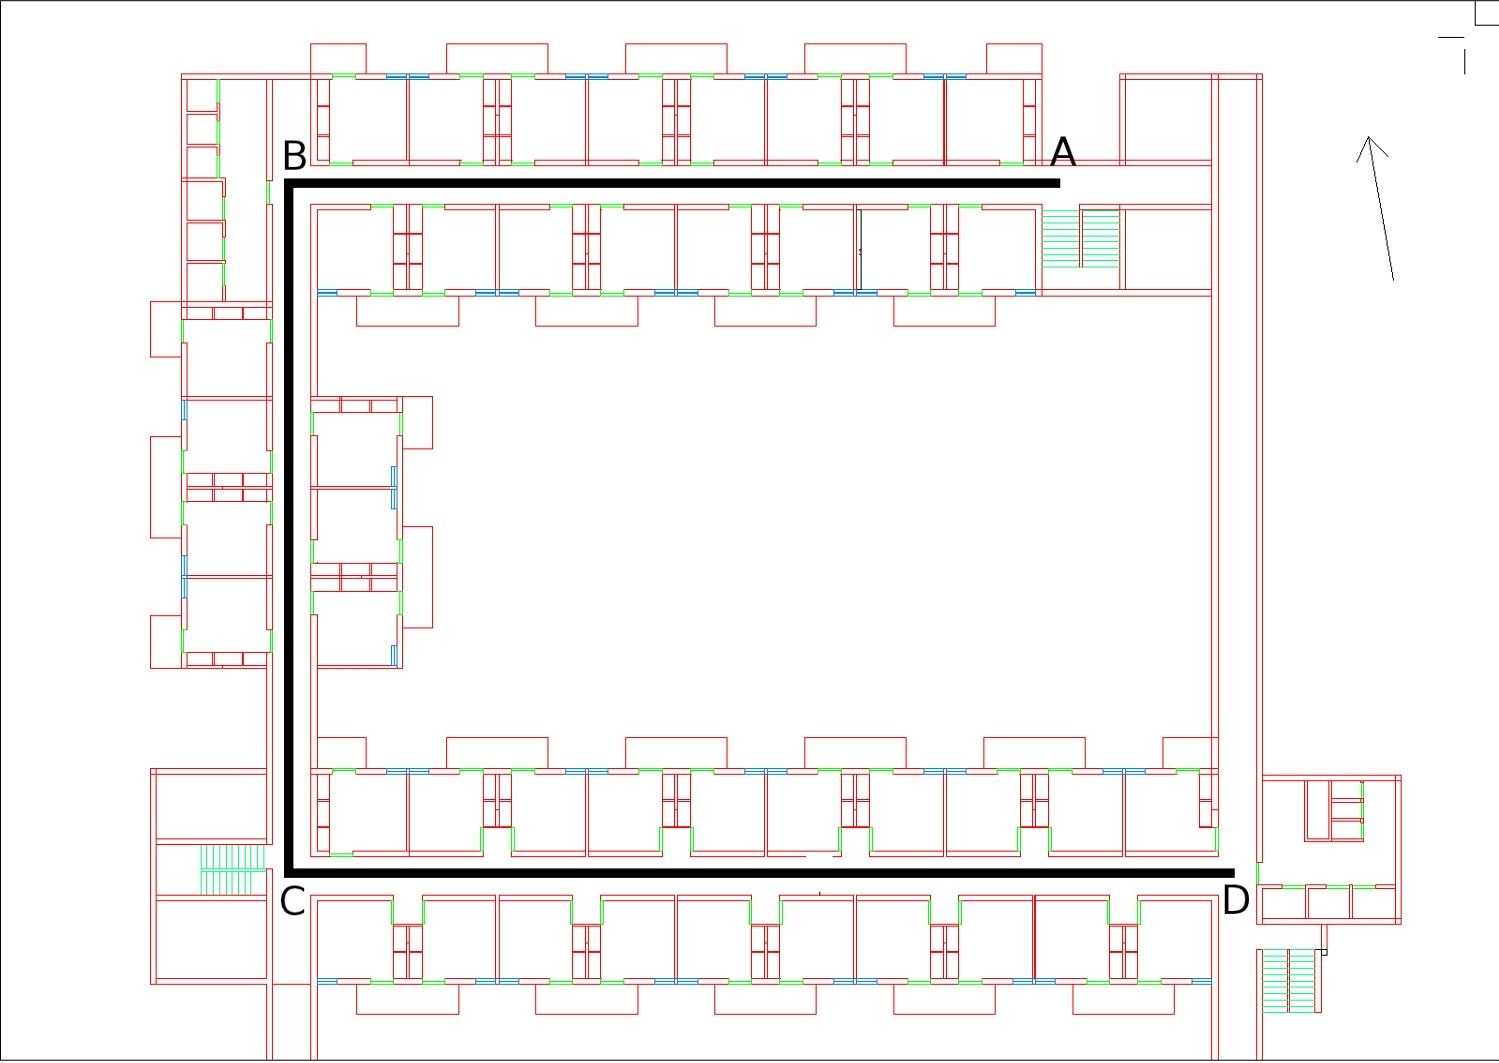
\includegraphics[width=5in]{figures/test_paths.jpg}
    \caption{Test paths for algorithm\label{fig:test_paths}}
\end{figure}


\section{Simple Dead Reckoning}

As discussed in the Literature Review (Chapter \ref{chap:literature_review}) and
in the Proposed Work (Chapter \ref{chap:proposed_method}), it is impossible to
directly obtain displacement information by double integration of the
accelerometer data. Hence, the step detection method was employed for tracking
the motion of the device as held by a walking human. The steps are integrated
with orientation information received from the magnetometer to create a 
simple dead reckoning system in accordance with the dynamical equation 
\eqref{eq:dr_eq}. The initial position for dead reckoning was obtained via
QRCodes in accordance with the description in Section \ref{sec:QRCodes}.
This algorithm is a control algorithm to be used for comparison with 
the proposed method.

\subsection{Simple Dead Reckoning Results}

One of the well known weaknesses of the dead reckoning approach is that it
diverges quickly from the ground truth unless corrective measures are taken.
As a basic control for the results, a simple dead reckoning based 
tracking algorithm was developed. 

Figure \ref{fig:dr_path1} shows the quick divergence of the algorithm
from the expected path A-B. In fact, at the end of a simple straight walk of 
around $30 m$, the estimate for the location has diverged a lot from the 
actual location. It should also be noted that the path taken passes through
rooms and walls and thus, doesn't look like a natural path for the user.

Figure \ref{fig:dr_path5} shows the extreme divergence that takes place 
over long distances. Table \ref{tbl:dr_error_growth} chronicles the 
error growth that takes place for this path at the turning points of the path.
It is amply clear that Simple Dead Reckoning is not suitable for tracking
if implemented as-is.

\begin{table}[bph]
\centering
\begin{tabular}{l c c}
\hline
\hline
Location    & Distance Travelled    & Error \\
\hline
A           & 0                     & 0 \\
B           & 30 m                  & 3.761 m \\
C           & 56 m                  & 4.982 m \\
D           & 92 m                  & 5.416 m \\
\hline
\end{tabular}
\caption{Error growth over distance for Simple Dead Reckoning\label{tbl:dr_error_growth}}
\end{table}

\begin{figure}
    \centering
    \includegraphics[width=4in]{figures/dr_path1}
    \caption{Performance of Dead Reckoning for Test Path 1\label{fig:dr_path1}}
\end{figure}
 
\begin{figure}
    \centering
    \includegraphics[width=4in]{figures/dr_path5}
    \caption{Performance of Dead Reckoning for Test Path 5\label{fig:dr_path5}}
\end{figure}
 
 

\section{Reckoning with NN Wifi correction}

As per our groundwork described in Section \ref{sec:knn_pos} we know that the 
mean error for positioning using KNN is around $2.8 m$ with a standard deviation
that is nearly the same as the mean. Given the large errors incurred by 
the dead reckoning solution, we wish to analyze the performance of Dead 
Reckoning after Wifi data is integrated into the system.

\subsection{Wifi Survey}

We carried out a Wifi Survey of the test area and collected 1562 samples by 
carefully laying down a $1 m \times 1 m$ grid and collected samples. 8
different samples were collected per grid point at orientations that were
detected to be 45 degrees apart by the onboard magnetometer. By relying on
the magnetometer itself to specify orientation, the effect of local magnetic
fields was taken into account during the survey. However, sensor noise causes
the angle values actually recorded with the Wifi Signal Strength data to vary 
from the expected orientation of the user.

\subsection{Tracking Performance}

While implementing and testing out the implementation of the KNN based 
tracking solution, the resource and scaling limitations of the system 
came to fore. 

Because of it being a ``lazy" algorithm that consults the entire 
training dataset on every query for a position, the KNN algorithm
is computationally very intensive. Queries for obtaining a position based
on Wifi information was a slow process that even disrupted the UI of the 
application due to its heavy workload. Optimizations involving cacheing 
of data and short-circuiting the distance calculation step based on the 
orientation angle of the training sample viz a viz the current device 
orientation were implemented. With these optimizations, we were able 
to successfully run a hybrid Dead Reckoning system that utilized 
Wifi Access Point Received Signal Strengths and Step motion information
to track the device.

The performance of the algorithm was again judged based on the test paths
mentioned in Section \ref{sec:test_paths}. Table \ref{tbl:NN_error} describes
the statistical nature of the error incurred for Path 1 with respect to the
actual position of the device. The values obtained agree with those reported in
papers like \cite{Wang} as well as our groundwork. Figure \ref{fig:nn_path1}
shows the track for Test path 1. A quick glance will indicate that the tracked
endpoints are reasonably accurate ($error$ $< 2 m$), however, the subjective nature
of the tracked path is very poor.

\begin{table}
\centering
\begin{tabular}{l c}
\hline
\hline
 & Error Value (m)\\
\hline
Min & 1.888e-07\\
$1^{st}$ Quartile & 1.448\\
Median & 2.948\\
Mean  & 3.748\\
$3^{rd}$ Quartile & 5.064\\
 Max.   & 14.87\\
Std. Dev. & 2.953\\
\hline
\end{tabular}
\caption{Error in tracking for the NN Algorithm\label{tbl:NN_error}}
\end{table}

\begin{figure}
    \centering
    \includegraphics[width=5in]{figures/nn_path1}
    \caption{Performance of the KNN algorithm for Test Path 1\label{fig:nn_path1}}
\end{figure}

\begin{figure}
    \centering
    \includegraphics[width=5in]{figures/nn_path5}
    \caption{Performance of the KNN algorithm for Test Path 5\label{fig:nn_path5}}
\end{figure}


%\subsection{Case 2: Dead reckoning with KNN averaging}
%\subsection{Case 3: Dead reckoning with clamped wifi positioning}

\section{Reckoning with Integrated Map Information}

The results of the Wifi corrected reckoning as well as the data collected 
as part of the implementation of the KNN positioning system indicates that 
the location information utilizing Wifi data is very unstable. On the other
hand there is significant drift if we depend solely on the accelerometer
and the magnetometer to provide intertial tracking. In order to get 
better accuracy from the system, we require constant feedback from the 
environment. A way to achieve that is to use the fact that the device 
holder is always moving through ``passable" spaces on the map. Any motion
contrary to the allowed locations on the map would indicate tracking drift 
and a feedback loop would be set up to correct for such errors.

In this context, the particle filter's performance is analyzed with the
same test tracks as the other two algorithms. 

As can be seen amply in Figure \ref{fig:pf_path2} and Figure \ref{fig:pf_path4}
the tracking performance of this algorithm is excellent. The drift errors of the 
dead reckoning solution are compensated for by the map information
which ensures that only states consistent with the motion of the device 
are retained. Long term behaviour of the algorithm is also remarkably 
stable. Even after moving close to 100 m, the algorithm was able to 
maintain a tracking error of less than 1 m. This is illustrated in 
Figure \ref{fig:pf_path4}.

To analyze the algorithm more carefully, the ground truth was 
mathematically modelled as a series of even sized steps along the path A-B
for a test done on Path 1. The resulting tracking errors were determined 
and their statistical analysis was done. The error distribution over the 
distance of 30 m are summarized in Table \ref{tbl:tracking_error}.

\begin{table}
\centering
\begin{tabular}{c c}
\hline
\hline
& Error Value (m)\\
\hline
 Min.    & 1.888e-07\\
 $1^{st}$ Quartile & 0.2750\\  
 Median  & 0.5218\\  
 Mean    & 0.5064\\  
 $3^{rd}$ Quartile & 0.7209\\  
 Max.    & 0.9412\\  
 Std. Dev.  & 0.2391\\
\hline
\end{tabular}
\caption{Tracking Error of Proposed Algorithm for Path 1\label{tbl:tracking_error}}
\end{table}

As is clear from this error distribution, the error incurred is low. Also, 
more importantly, the standard deviation of the error distribution is low.
Hence it is unlikely that we will get large deviations from the tracked path.

\begin{figure}
    \centering
    \includegraphics[width=5in]{figures/pf_path2}
    \caption{Performance of Reckoning with Map info for Test Path 2.\label{fig:pf_path2}}
\end{figure}

\begin{figure}
    \centering
    \includegraphics[width=5in]{figures/pf_path4}
    \caption{Performance of the Reckoning algorithm for Test Path 4.\label{fig:pf_path4}}
\end{figure}


\section{Recovery from Particle Insufficiency}

For a typical test path, the variation in the number of live particles is 
shown in Figure \ref{fig:live_particles}. As can be seen clearly, the 
particle filter does suffer dips in the number of live particles but the 
number of particles remaining is around 5. Thus maximum value of 50 particles 
seems to be a reasonable value for our tracking algorithm. An empirical 
determination of the computational limits of the implemented algorithm 
seems to indicate that the maximum number of particles that the 
device is able to update per computation step lies around 200. 

\begin{figure}
    \centering
    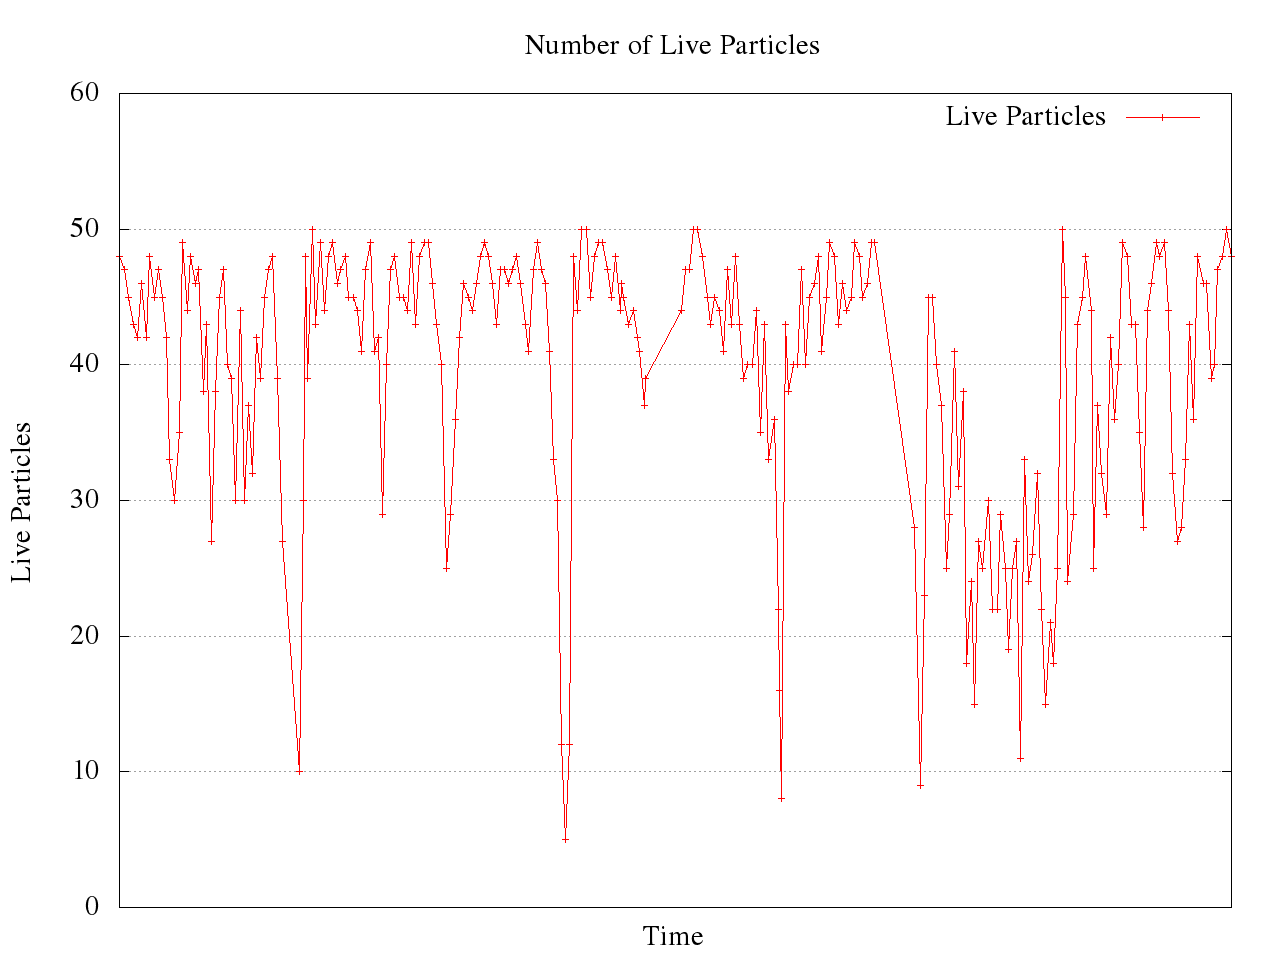
\includegraphics{figures/live_particles.png}
    \caption{Number of Live Particles for a Path\label{fig:live_particles}}
\end{figure}

The dips seen in Figure \ref{fig:live_particles} correspond to events where 
the particle filter is adapting its location estimate based on feedback 
received from $MapSelect$. The algorithm may get lost if the dips 
reach a value 0. In this case the recovery algorithm is invoked.
Figure \ref{fig:recovery_result} shows how the particle filter 
recovered successfully from a ``lost" scenario to continue tracking of the 
device, albeit with some error.

\begin{figure}
    \centering
    \includegraphics{figures/recovery_result.png}
    \caption{Result of a successful recovery\label{fig:recovery_result}}
\end{figure}


\section{Comparison with published results}

With additional information at hand as well as suitable modifications to the 
dynamical equations of the system and care in avoiding particle degeneracy,
a significantly better accuracy has been achieved by this system as compared
to previous published works. 

The comparison of the 3 implemented methods is shown in Table \ref{tbl:pub_comparison}.


\begin{table}
\centering
\begin{tabular}{l c c}
\hline
\hline
Algorithm & Mean Error (m) & Std. Dev. (m)\\
\hline
Wang\cite{Wang} KNN only & 6.44 & 6.84\\
Wang\cite{Wang} PF with RSSI & 5.57 & 3.9\\
Wang\cite{Wang} PF with RSSI + Steps & 4.54 & 3.52\\
Wang\cite{Wang} PF with RSSI + Steps + Map & 4.30 & 2.80\\
Evennou\cite{Evennou} PF with RSSI & 1.86 & N/A\\
Evennou\cite{Evennou} PF with RSSI + INS & 1.53 & N/A\\
\textbf{Control Algorithm: NN Wifi corrected Reckoning} & \textbf{3.748} & \textbf{2.953}\\
\textbf{Proposed Work: PF with INS + Map} & \textbf{0.5064} & \textbf{0.2391}\\
\hline
\end{tabular}
\caption{Comparison with Published Results\label{tbl:pub_comparison}}
\end{table} 

\section{Complete listing of the results}

In order to maintain the flow of the thesis and due to the voluminous
nature of reporting the results for each of the test paths for the 3
algorithms, the results of those tests have been reported in the appendices.

%\missingfigure{CDF of the errors of the methods (will take some time)}



\chapter{Summary and Future Work\label{chap:summary}}
Use and evaluation of SVM as a suitable architecture for the Wifi data.
Better integration of information from the camera.
Integration of information using a Barometric sensor would be useful for detecting elevation changes. A system for the same is proposed but the experimental results were not obtained. 


\section{Particle filter + Wifi data}

\subsection{Case 1: Use of Wifi data for accounting for drift errors}
\subsection{Case 2: Use of Oriented Wifi data for accounting for drift errors}
\subsection{Case 3: Use of clamped wifi data for accounting for drift errors}
\subsection{Case 4: Use of area Restricted Wifi data for accounting for drift errors}
\subsection{Case 7: Simple post processing of output.??}

\section{Signal Strength Map}

TODO if time permits
Wifi signal strength map developed using crowdsourced data for use in systems such as RedPin.


\section{Integration of barometric information}

\section{Exploration of crowdsourcing Wifi data}

\section{Analysis of Wifi signal strength distribution}




\appendix

%\todo[inline]{Enable this appendix later}
\chapter{Test results for all algorithms}

\section{Simple Dead Reckoning}

\begin{figure}
    \centering
    \includegraphics[width=3in]{figures/sdr_path1}
    \caption{Simple Dead Reckoning Path 1\label{fig:sdr_path1}}
\end{figure}

\begin{figure}
    \centering
    \includegraphics[width=3in]{figures/sdr_path2}
    \caption{Simple Dead Reckoning Path 2\label{fig:sdr_path2}}
\end{figure}

\begin{figure}
    \centering
    \includegraphics[width=3in]{figures/sdr_path3}
    \caption{Simple Dead Reckoning Path 3\label{fig:sdr_path3}}
\end{figure}

\begin{figure}
    \centering
    \includegraphics[width=3in]{figures/sdr_path4}
    \caption{Simple Dead Reckoning Path 4\label{fig:sdr_path4}}
\end{figure}

\begin{figure}
    \centering
    \includegraphics[width=3in]{figures/sdr_path5}
    \caption{Simple Dead Reckoning Path 5\label{fig:sdr_path5}}
\end{figure}

\section{Wifi Corrected Reckoning}

\begin{figure}
    \centering
    \includegraphics[width=3in]{figures/wcr_path1}
    \caption{Wifi Corrected Reckoning Path 1\label{fig:wcr_path1}}
\end{figure}

\begin{figure}
    \centering
    \includegraphics[width=3in]{figures/wcr_path2}
    \caption{Wifi Corrected Reckoning Path 2\label{fig:wcr_path2}}
\end{figure}

\begin{figure}
    \centering
    \includegraphics[width=3in]{figures/wcr_path3}
    \caption{Wifi Corrected Reckoning Path 3\label{fig:wcr_path3}}
\end{figure}

\begin{figure}
    \centering
    \includegraphics[width=3in]{figures/wcr_path4}
    \caption{Wifi Corrected Reckoning Path 4\label{fig:wcr_path4}}
\end{figure}

\begin{figure}
    \centering
    \includegraphics[width=3in]{figures/wcr_path5}
    \caption{Wifi Corrected Reckoning Path 5\label{fig:wcr_path5}}
\end{figure}


\section{Reckoning with Map Information}

\begin{figure}
    \centering
    \includegraphics[width=3in]{figures/mcr_path1}
    \caption{Reckoning with Map Information Path 1\label{fig:mcr_path1}}
\end{figure}

\begin{figure}
    \centering
    \includegraphics[width=3in]{figures/mcr_path2}
    \caption{Reckoning with Map Information Path 2\label{fig:mcr_path2}}
\end{figure}

\begin{figure}
    \centering
    \includegraphics[width=3in]{figures/mcr_path3}
    \caption{Reckoning with Map Information Path 3\label{fig:mcr_path3}}
\end{figure}

\begin{figure}
    \centering
    \includegraphics[width=3in]{figures/mcr_path4}
    \caption{Reckoning with Map Information Path 4\label{fig:mcr_path4}}
\end{figure}

\begin{figure}
    \centering
    \includegraphics[width=3in]{figures/mcr_path5}
    \caption{Reckoning with Map Information Path 5\label{fig:mcr_path5}}
\end{figure}



%\chapter{Survey Form}


\backmatter

\singlespace
\bibliographystyle{IEEEtran}
\addcontentsline{toc}{chapter}{Bibliography}
\bibliography{IEEEfull,mybib}


\end{document}
